% Options for packages loaded elsewhere
\PassOptionsToPackage{unicode}{hyperref}
\PassOptionsToPackage{hyphens}{url}
\PassOptionsToPackage{dvipsnames,svgnames,x11names}{xcolor}
%
\documentclass[
  12pt,
]{article}

\usepackage{amsmath,amssymb}
\usepackage{iftex}
\ifPDFTeX
  \usepackage[T1]{fontenc}
  \usepackage[utf8]{inputenc}
  \usepackage{textcomp} % provide euro and other symbols
\else % if luatex or xetex
  \usepackage{unicode-math}
  \defaultfontfeatures{Scale=MatchLowercase}
  \defaultfontfeatures[\rmfamily]{Ligatures=TeX,Scale=1}
\fi
\usepackage{lmodern}
\ifPDFTeX\else  
    % xetex/luatex font selection
\fi
% Use upquote if available, for straight quotes in verbatim environments
\IfFileExists{upquote.sty}{\usepackage{upquote}}{}
\IfFileExists{microtype.sty}{% use microtype if available
  \usepackage[]{microtype}
  \UseMicrotypeSet[protrusion]{basicmath} % disable protrusion for tt fonts
}{}
\makeatletter
\@ifundefined{KOMAClassName}{% if non-KOMA class
  \IfFileExists{parskip.sty}{%
    \usepackage{parskip}
  }{% else
    \setlength{\parindent}{0pt}
    \setlength{\parskip}{6pt plus 2pt minus 1pt}}
}{% if KOMA class
  \KOMAoptions{parskip=half}}
\makeatother
\usepackage{xcolor}
\usepackage[left=1in,right=1in,top=1in,bottom=1in]{geometry}
\setlength{\emergencystretch}{3em} % prevent overfull lines
\setcounter{secnumdepth}{5}
% Make \paragraph and \subparagraph free-standing
\ifx\paragraph\undefined\else
  \let\oldparagraph\paragraph
  \renewcommand{\paragraph}[1]{\oldparagraph{#1}\mbox{}}
\fi
\ifx\subparagraph\undefined\else
  \let\oldsubparagraph\subparagraph
  \renewcommand{\subparagraph}[1]{\oldsubparagraph{#1}\mbox{}}
\fi


\providecommand{\tightlist}{%
  \setlength{\itemsep}{0pt}\setlength{\parskip}{0pt}}\usepackage{longtable,booktabs,array}
\usepackage{calc} % for calculating minipage widths
% Correct order of tables after \paragraph or \subparagraph
\usepackage{etoolbox}
\makeatletter
\patchcmd\longtable{\par}{\if@noskipsec\mbox{}\fi\par}{}{}
\makeatother
% Allow footnotes in longtable head/foot
\IfFileExists{footnotehyper.sty}{\usepackage{footnotehyper}}{\usepackage{footnote}}
\makesavenoteenv{longtable}
\usepackage{graphicx}
\makeatletter
\def\maxwidth{\ifdim\Gin@nat@width>\linewidth\linewidth\else\Gin@nat@width\fi}
\def\maxheight{\ifdim\Gin@nat@height>\textheight\textheight\else\Gin@nat@height\fi}
\makeatother
% Scale images if necessary, so that they will not overflow the page
% margins by default, and it is still possible to overwrite the defaults
% using explicit options in \includegraphics[width, height, ...]{}
\setkeys{Gin}{width=\maxwidth,height=\maxheight,keepaspectratio}
% Set default figure placement to htbp
\makeatletter
\def\fps@figure{htbp}
\makeatother
\newlength{\cslhangindent}
\setlength{\cslhangindent}{1.5em}
\newlength{\csllabelwidth}
\setlength{\csllabelwidth}{3em}
\newlength{\cslentryspacingunit} % times entry-spacing
\setlength{\cslentryspacingunit}{\parskip}
\newenvironment{CSLReferences}[2] % #1 hanging-ident, #2 entry spacing
 {% don't indent paragraphs
  \setlength{\parindent}{0pt}
  % turn on hanging indent if param 1 is 1
  \ifodd #1
  \let\oldpar\par
  \def\par{\hangindent=\cslhangindent\oldpar}
  \fi
  % set entry spacing
  \setlength{\parskip}{#2\cslentryspacingunit}
 }%
 {}
\usepackage{calc}
\newcommand{\CSLBlock}[1]{#1\hfill\break}
\newcommand{\CSLLeftMargin}[1]{\parbox[t]{\csllabelwidth}{#1}}
\newcommand{\CSLRightInline}[1]{\parbox[t]{\linewidth - \csllabelwidth}{#1}\break}
\newcommand{\CSLIndent}[1]{\hspace{\cslhangindent}#1}

% \usepackage{changebar}
% \usepackage[T1]{fontenc}
% \usepackage[utf8]{inputenc}


\usepackage{setspace}
\usepackage{amsmath,amssymb,graphicx,rotating,float}
\usepackage{tikz-cd}

% \usepackage[T1]{fontenc}
% \setmainfont[Numbers={Lining,Proportional,OldStyle}]{Minion3}
% \usepackage{mathpazo}
% \usepackage{MinionPro}

\usepackage{mathptmx}
% \usepackage{helvet}

% \usepackage[symbol]{footmisc}

% \renewcommand{\thefootnote}{\fnsymbol{footnote}}

% \usepacakge{mathspec}
% \usepackage[compact]{titlesec}  
% \usepackage{bm}
% 
% \defaultfontfeatures{Ligatures=TeX}


% \setmainfont[Numbers={Lining,Proportional,OldStyle}]{Minion3}
% \setmainfont[
% Numbers={Lining,Proportional,OldStyle},
% ItalicFeatures={Scale=1.05}
% ]{Cochineal}
% \usepackage{unicode-math}

% \setmathfont[version=bold]{MinionMath-Bold}

% \setmathfont[
%     Extension = .otf,
%     Scale = 1,
%     Script = Math,
%     SizeFeatures = {
%             {Size = -6, Font = MinionMath-Tiny,
%               Style = MathScriptScript},
%             {Size = 6-8.4, Font = MinionMath-Capt,
%               Style = MathScript},
%             {Size = 8.4-, Font = MinionMath-Regular},
%     },
%     ]{MinionMath-Regular}
% \setmathfont[range={\mathfrak}]{latinmodern-math.otf}
% \setmathfont[range={\mathcal}]{latinmodern-math.otf}
% \setmathfont[range={\mathscr}]{latinmodern-math.otf}
% \let\svmathcal\mathcal
% \DeclareSymbolFontAlphabet{\mathcal}{symbols}
% \DeclareMathAlphabet{\mathcal}{OMS}{cmsy}{m}{n}
% \SetMathAlphabet{\mathcal}{bold}{OMS}{cmsy}{b}{n}

% \setmathfont[range={"0041-"005A,"0061-"007A,"D434-"D467}]{Cochineal}
% \setmathfont[range={"D434-"D467}]{Cochineal Italic}
% \setmathfont[range={"D468-"D49B}]{Cochineal Bold Italic}



% \setmathfont[range=it]{Cochineal Italic}
% \setmathfont[range=bfup]{Cochineal Bold}
% \setmathfont[range=bfit]{Cochineal Bold Italic}
% \setmathfont[range={}]{Minion Math}
% \setmonofont[Scale=0.85]{Ubuntu Mono}
% \setmonofont[Scale=0.85]{Fira Code}
% \setmonofont[Scale=0.83]{Operator Mono}
% \setsansfont[Scale=0.90]{PT Sans}
% \titleformat{\chapter}[display]{\sffamily\huge\bfseries}{\chaptertitlename\ \thechapter}{20pt}{\Huge}


% \usepackage{microtype}
% \usepackage{hyperref}

\usepackage{xcolor}
\definecolor{myred}{RGB}{140, 26, 17}
\definecolor{myblue}{RGB}{42, 45, 116}
\definecolor{mygray}{RGB}{100, 100, 100}
\definecolor{uoiblue}{HTML}{13294B}
\definecolor{uoiorange}{HTML}{FF5F05}
\definecolor{uoiorange2}{HTML}{C84113}
\definecolor{ucladarkblue}{HTML}{005587}

% \usepackage{titling}
% \pretitle{\begin{flushleft}\huge\bfseries}
% \posttitle{\end{flushleft}}
% \preauthor{\begin{flushleft}\Large}
% \postauthor{\end{flushleft}}
% \predate{\begin{flushleft}\large}
% \postdate{\end{flushleft}}

% \makeatletter         
% \def\@maketitle{   % custom maketitle 
% \sffamily \hfill \small {\@date} 
% \smallskip \hrule \bigskip 

% \vspace*{3cm}
% {
% {\LARGE  \bfseries \@title \\ \vspace*{1cm}}
% {\@author\\}
% {\footnotesize \tt \href{mailto:jhchae2@illinois.edu}{jhchae2@illinois.edu}}
% }
% }

% \hypersetup{colorlinks=true, linkcolor=myred, urlcolor=myred, citecolor=myred, anchorcolor=myred}


% \let\paragraph\oldparagraph
% \let\subparagraph\oldsubparagraph

% now my mods
% \usepackage{titlesec, blindtext, color}
% etc etc
% \renewcommand{\paragraph}[1]{\oldparagraph{#1}\mbox{}\par}
% \titleformat*{\section}{\sffamily\Large\bfseries}
% \titleformat*{\subsection}{\sffamily\bfseries}
% \titleformat*{\subsubsection}{\sffamily\itshape}
% \titleformat*{\paragraph}{\sffamily\bfseries}

% \newcommand{\doctitle}{News Frames of Inflation Issue}
% \newcommand{\myname}{Je Hoon Chae}
% \newcommand{\myemail}{jhchae2@illinois.edu}
% \newcommand{\course}{Gov 2001: Quantitative Social Science Methods I}
% \newcommand{\headertitle}{Gov 2001: \psetnum}
% \newcommand{\mydepartment}{\itshape Department of Communication}
% \newcommand{\myinstitution}{\itshape University of Illinois at Urbana-Champaign}

% Header setting
% \usepackage{fancyhdr}
% \pagestyle{fancy}
% \fancyhead[L]{\footnotesize\sffamily Gov 2001: Problem Set 3} % upper-left
% \fancyhead[L]{\footnotesize\sc Gov 2001: \psetnum} % upper-left
% \fancyhead[R]{\footnotesize\sc\nouppercase{\leftmark}} % upper-right
% \fancyfoot[c]{\small\thepage} % page number

% \usepackage{titling}
% \setlength{\droptitle}{5cm}
% Make title new setting
% \renewcommand{\maketitle}{%
%   \begin{center}
%   {\Large\@author}\par
%   \vspace*{\fill}
%   {\Huge\textbf{\@title}}\par
%   \vspace*{\fill}
%   \@date
%   \end{center}
% }

% \renewcommand\maketitle{
%     \vspace*{1cm}
%     \begin{flushleft}
%         {\setstretch{1.2}
%         {\LARGE\bfseries\doctitle\\ \vspace{0.5cm}}
%         {\large\myname \\}
%         % {\mydepartment \\}
%         {\myinstitution \\}
%         {\footnotesize \tt \href{mailto:\myemail}{\myemail}}
%         }
%     \end{flushleft}
% }
% \DeclareOldFontCommand{\bf}{\normalfont\bfseries}{\mathbf}

% \usepackage{fancyhdr, lastpage}
% \setcounter{secnumdepth}{0}

% \newcommand{\RomanNumeralCaps}[1]{\MakeUppercase{\romannumeral #1}}
% \newcommand{\inv}{^{\hspace{0.6mm}-1}}
% \newcommand*\diff{\mathop{}\!\mathrm{d}}
% \newcommand*\bvec[1]{\vec{\mathbf{#1}}}
% \newcommand*\lvec[1]{\overrightarrow{\mathbf{#1}}}
% \newcommand{\var}{\mathbb{V}\text{ar}}

% \newcommand*\lbox[1]{\fcolorbox{black}{black!2}{\begin{minipage}{0.98\textwidth}{#1}\end{minipage}}}
\makeatletter
\makeatother
\makeatletter
\makeatother
\makeatletter
\@ifpackageloaded{caption}{}{\usepackage{caption}}
\AtBeginDocument{%
\ifdefined\contentsname
  \renewcommand*\contentsname{Table of contents}
\else
  \newcommand\contentsname{Table of contents}
\fi
\ifdefined\listfigurename
  \renewcommand*\listfigurename{List of Figures}
\else
  \newcommand\listfigurename{List of Figures}
\fi
\ifdefined\listtablename
  \renewcommand*\listtablename{List of Tables}
\else
  \newcommand\listtablename{List of Tables}
\fi
\ifdefined\figurename
  \renewcommand*\figurename{Figure}
\else
  \newcommand\figurename{Figure}
\fi
\ifdefined\tablename
  \renewcommand*\tablename{Table}
\else
  \newcommand\tablename{Table}
\fi
}
\@ifpackageloaded{float}{}{\usepackage{float}}
\floatstyle{ruled}
\@ifundefined{c@chapter}{\newfloat{codelisting}{h}{lop}}{\newfloat{codelisting}{h}{lop}[chapter]}
\floatname{codelisting}{Listing}
\newcommand*\listoflistings{\listof{codelisting}{List of Listings}}
\makeatother
\makeatletter
\@ifpackageloaded{caption}{}{\usepackage{caption}}
\@ifpackageloaded{subcaption}{}{\usepackage{subcaption}}
\makeatother
\makeatletter
\@ifpackageloaded{tcolorbox}{}{\usepackage[skins,breakable]{tcolorbox}}
\makeatother
\makeatletter
\@ifundefined{shadecolor}{\definecolor{shadecolor}{rgb}{.97, .97, .97}}
\makeatother
\makeatletter
\makeatother
\makeatletter
\ifdefined\Shaded\renewenvironment{Shaded}{\begin{tcolorbox}[enhanced, borderline west={3pt}{0pt}{shadecolor}, sharp corners, frame hidden, boxrule=0pt, breakable, interior hidden]}{\end{tcolorbox}}\fi
\makeatother
\makeatletter
\makeatother
\ifLuaTeX
  \usepackage{selnolig}  % disable illegal ligatures
\fi
\IfFileExists{bookmark.sty}{\usepackage{bookmark}}{\usepackage{hyperref}}
\IfFileExists{xurl.sty}{\usepackage{xurl}}{} % add URL line breaks if available
\urlstyle{same} % disable monospaced font for URLs
\hypersetup{
  pdftitle={Fact-Checking and Partisan Cheerleading: Dissemination Patterns of Political Fact-Checks on Twitter},
  pdfauthor={Je Hoon Chae},
  colorlinks=true,
  linkcolor={ucladarkblue},
  filecolor={Maroon},
  citecolor={Blue},
  urlcolor={ucladarkblue},
  pdfcreator={LaTeX via pandoc}}

\title{Fact-Checking and Partisan Cheerleading: Dissemination Patterns
of Political Fact-Checks on Twitter\footnote{Author thanks to Pablo
  Barberá for generously sharing data. Also, author thanks to Sakshi
  Bhalla, Mengqing (Maggie) Zhang, Nino Migineishvili, Jonghyun Lee, and
  Joyce Yanru Jiang for their help for the data collection.
  Additionally, author thanks to David Tewksbury, Tim Groeling, Briony
  Swire-Thompson, Eehyun Kim, Junmo Song, Jina Lee, and Soomin Hong for
  their helpful comments on the study.}}
\usepackage{etoolbox}
\makeatletter
\providecommand{\subtitle}[1]{% add subtitle to \maketitle
  \apptocmd{\@title}{\par {\large #1 \par}}{}{}
}
\makeatother
\subtitle{5995 words (excluding references)}
\author{Je Hoon Chae\footnote{Doctoral Student, Department of
  Communication, University of California, Los Angeles. email:
  \href{mailto:chae@g.ucla.edu}{chae@g.ucla.edu}. webpage:
  \href{https://jehoonchae.github.io}{https://jehoonchae.github.io}}}
\date{July 27, 2023}

\begin{document}
\maketitle
\begin{abstract}
\noindent In this study, we delve into the dynamics of political
fact-checking news dissemination using an extensive dataset of
PolitiFact articles and associated Twitter posts spanning from 2016 to
2021. We focus on how fact-checking content, whether aligned or
conflicting with individual beliefs, penetrates across partisan divides.
Our analysis reveals a strong tendency for fact-checking verdicts to
favor Liberal/Democratic predispositions, a trend that amplifies during
election cycles, while this trend doesn't directly imply a political
bias in the fact-checking organization, since favorability distributions
in published content cannot solely determine biases. Additionally, we
find that Twitter users sharing fact-checking news predominantly align
with liberal ideologies, regardless of the congruency of the fact-check
result. The data shows an increase in the sharing of fact-checking
content in alignment with users' political ideology during elections,
with a significant spike among liberal users. Moreover, we unearth a
substantial disparity in the sharing behavior among Twitter users, with
a handful of heavy users dominating the dissemination landscape.
Importantly, we uncover a clear connection between a user's political
ideology and their tendency to selectively share content, a pattern
especially pronounced among conservative users.
\end{abstract}
\setlength{\parindent}{20pt}
\setlength{\parskip}{0pt}

\newpage

\doublespacing

\hypertarget{introduction}{%
\section{Introduction}\label{introduction}}

Fact-checking organizations serve a crucial role in our information
landscape, tirelessly evaluating the truthfulness of statements made by
public figures, celebrities, and relevant social media posts alike
(\protect\hyperlink{ref-graves2016}{Graves, 2016}). In the United
States, a diverse range of organizations---from specialized
fact-checking groups such as \emph{PolitiFact}, \emph{FactCheck.org},
and \emph{Snopes}, to well-known news agencies like \emph{CNN},
\emph{The Washington Post}, \emph{NPR}, and \emph{The New York
Times}---are committed to verifying the authenticity of these
declarations. More specifically, organizations like \emph{PolitiFact}
devote considerable resources to evaluating the veracity of assertions
within the political landscape.

The process of claim adjudication in political sphere has undoubtedly
ignited numerous debates, such as triggering partisan motivated
reasoning or allegations of political bias contingent on the result of
fact-checking. However, empirical evidence suggests that individuals
reliably amend their perceptions in line with fact-checking outcomes
(\protect\hyperlink{ref-nyhan2020taking}{Nyhan et al., 2020};
\protect\hyperlink{ref-porter2022factual}{Porter et al., 2022};
\protect\hyperlink{ref-porter2022political}{Porter \& Wood, 2022};
\protect\hyperlink{ref-swire2017processing}{Swire et al., 2017};
\protect\hyperlink{ref-swire2020they}{Swire-Thompson et al., 2020};
\protect\hyperlink{ref-walter2020fact}{Walter et al., 2020}). This
effect remains durable even when the information provided by the
fact-check contradicts previously held beliefs
(\protect\hyperlink{ref-coppock2023conceptual}{Coppock et al., 2023};
\protect\hyperlink{ref-wood2019elusive}{Wood \& Porter, 2019}) or the
fact-checking source is considered to be an out-group
(\protect\hyperlink{ref-chae2023perceiving}{Chae et al., 2023}). Such
findings offer a glimmer of optimism, suggesting that even staunch
partisans may be capable of rational evaluation of disputed factual
information. However, this raises the question: does exposure to
cross-cutting fact-checking news genuinely occur in everyday life?

While a considerable body of academic research has assessed the
effectiveness of fact-checking within controlled experimental settings,
our grasp of fact-checking consumption within real-world contexts
remains insufficient. One notable exception is the recent study by Guess
et al. (\protect\hyperlink{ref-guess2020exposure}{2020}), which
leveraged a mix of survey responses and web search tracking data. This
investigation established that direct visits to fact-checking websites
are extraordinarily infrequent, leaving the dynamics of cross-cutting
exposure largely under-researched. As a consequence, individuals rarely
access fact-checking news directly from specialized websites. This
outcome implies that in real-world scenarios, social media arguably
becomes the primary conduit for fact-checking news. This conclusion,
based on empirical evidence from the Guess et al.
(\protect\hyperlink{ref-guess2020exposure}{2020}) study, underscores the
crucial role of indirect or incidental exposure to fact-checking within
social media platforms
(\protect\hyperlink{ref-fletcher2018people}{Fletcher \& Nielsen, 2018}).
However, preliminary research using social media data from platforms
such as Twitter and Facebook suggests that these environments do not
offer ideal conditions for cross-cutting information consumption
(\protect\hyperlink{ref-bakshy2015exposure}{Bakshy et al., 2015};
\protect\hyperlink{ref-barbera2015tweeting}{Barberá et al., 2015};
\protect\hyperlink{ref-conover2011political}{Conover et al., 2011}).
Rather, these platforms appear highly susceptible to partisan selective
information sharing and exposure
(\protect\hyperlink{ref-bowen2023learning}{Bowen et al., 2023};
\protect\hyperlink{ref-osmundsen2021partisan}{Osmundsen et al., 2021}),
with fact-checking news not being immune to this pattern
(\protect\hyperlink{ref-shin2017partisan}{Shin \& Thorson, 2017}). If
cross-cutting fact-checking exposure does not frequently occur in
reality, then the meaningfulness of experimental findings demonstrating
the robustness of correction effects (e.g.,
\protect\hyperlink{ref-wood2019elusive}{Wood \& Porter, 2019}) against
the widespread perspective of partisan motivated reasoning
(\protect\hyperlink{ref-taber2006motivated}{Taber \& Lodge, 2006}) is
called into question.

In this regards, our study aims to examine the degree to which political
fact-checking news, either congruent (pro-attitudinal) or discordant
(counter-attitudinal) with individuals' beliefs, permeates partisan
boundaries. We aim to investigate whether this fact-checking content is
shared within and across partisan divides, potentially contributing to a
shared understanding of political reality. To achieve our research aims,
we capitalized on a comprehensive dataset comprised of all fact-checking
articles published by \emph{PolitiFact} (\(N = 9,523\))---a preeminent
fact-checking organization---from January 1, 2016, to December 31, 2021.
This corpus also encompassed the corresponding Twitter posts
(\(N = 35,965\)) and affiliated retweet information for each article
(\(N_{\text{users}} = 153,797\); \(N_{\text{retweet}} = 1,082,122\)).
Delving into this wealth of data, we distilled several key findings.

It was found that over 60\% of fact-checks deemed initial factual claims
as false, a number of which were from sources associated with the
Conservative/Republican Party. The study further discovered a greater
volume of fact-checks congruent with Liberal/Democrats than with
Conservative/Republicans throughout the period under investigation, with
a notable increase in activity leading up to elections. When it came to
dissemination, Twitter users sharing fact-checking news predominantly
leaned towards liberal ideologies, a skew which remained even when
conservative-leaning fact-checking content was included. Users sharing
Liberal/Democrat congruent fact-checking echoed the overall distribution
of fact-checking sharers, while conservative congruent fact-checking was
relatively more shared among conservative-leaning users. The study also
identified an increase in partisan-congruent sharing of fact-checking
content during election periods, particularly among liberal users. The
sharing of fact-checking posts was dominated by a small subset of heavy
users, revealing a significant disparity in the sharing behavior among
Twitter users. Lastly, the study highlighted selective sharing behavior,
where a user's political ideology positively correlated with the extent
of their selective sharing behavior, a trend more pronounced among
conservative users.

\hypertarget{partisan-selective-sharing-of-fact-checking-news-on-social-media}{%
\section{Partisan Selective Sharing of Fact-Checking News on Social
Media}\label{partisan-selective-sharing-of-fact-checking-news-on-social-media}}

We approach our understanding of how political fact-checking news is
shared on social media through the lens of the two-step flow
communication theory (\protect\hyperlink{ref-katz1957two}{Katz, 1957};
\protect\hyperlink{ref-katz1955personal}{Katz \& Lazarsfeld, 1955}). We
supplement this with insights from theories surrounding
partisan-motivated information processing
(\protect\hyperlink{ref-kunda1990case}{Kunda, 1990};
\protect\hyperlink{ref-stroud2010polarization}{Stroud, 2010};
\protect\hyperlink{ref-taber2006motivated}{Taber \& Lodge, 2006}). The
two-step flow communication theory posits that interpersonal
relationships, rather than direct interaction with the original sources,
usually convey media messages to the general public
(\protect\hyperlink{ref-katz1957two}{Katz, 1957}). In the realm of
fact-checking news on social media, these intermediary ``opinion
leaders'' (\protect\hyperlink{ref-lazarsfeld1944people}{Lazarsfeld et
al., 1944}) actively interact with fact-checking sites, digest
fact-checked posts early, and circulate the examined information within
their networks (\protect\hyperlink{ref-chadwick2011political}{Chadwick,
2011}; \protect\hyperlink{ref-kim2013stumbling}{Kim et al., 2013}).
Owing to their heightened political involvement, these individuals play
a crucial role in spreading news on social media
(\protect\hyperlink{ref-messing2014selective}{Messing \& Westwood,
2014}).

The emergence of social media platforms has magnified the importance of
the two-step flow theory. Prior research has found that most social
media users may not directly engage with fact-checking news, despite its
extensive availability (\protect\hyperlink{ref-guess2020exposure}{Guess
et al., 2020}). Instead, opinion leaders or heavy social media users
share this content within their networks, distributing the news
(\protect\hyperlink{ref-bode2016political}{Bode, 2016}). The
interpretation and presentation by these opinion leaders significantly
influence their network's acceptance or rejection of fact-checked
information (\protect\hyperlink{ref-bakshy2015exposure}{Bakshy et al.,
2015}). Moreover, the two-step flow theory highlights the existence of
echo chambers and information bubbles on social media. If opinion
leaders mainly share fact-checking news that aligns with their
ideological predispositions, their networks primarily get exposure to
this selectively presented information. This dynamic fosters echo
chambers and ideological polarization
(\protect\hyperlink{ref-barbera2015social}{Barberá, 2015b};
\protect\hyperlink{ref-flaxman2016filter}{Flaxman et al., 2016}).

Twitter and Facebook, as social media platforms, have expanded the
applicability of the two-step flow of communication theory. They serve
as perfect environments for opinion leaders to convey information to a
wide audience. For instance, a study on Twitter users during the 2016
U.S. election found that politically engaged individuals often spurred
the spread of political information
(\protect\hyperlink{ref-barbera2015tweeting}{Barberá et al., 2015}).
Individuals less politically engaged then shared and consumed this
distributed information. This pattern is a reflection of the two-step
flow of communication theory, where opinion leaders get information from
mass media and then broadcast it to their followers, shaping public
opinion (\protect\hyperlink{ref-barbera2015tweeting}{Barberá et al.,
2015}). Additionally, it was revealed that Facebook users with strong
partisan beliefs were more likely to share news articles that bolstered
their perspectives (\protect\hyperlink{ref-wells2016coproduction}{Wells
et al., 2016}). These partisan users disseminate news within their
social networks, influencing their less politically active friends' and
followers' views. This action represents the first step in the two-step
flow. The explicit display of the two-step flow of communication on both
Twitter and Facebook reaffirms the theory's relevance in today's digital
media landscape.

So, what are the psychological factors that drive individuals to
selectively share news on social media? Essentially, users' news sharing
behavior on social media is a self-presentation exercise
(\protect\hyperlink{ref-gantz1979people}{Gantz \& Trenholm, 1979};
\protect\hyperlink{ref-kraft2020social}{Kraft et al., 2020};
\protect\hyperlink{ref-walther1996computer}{Walther, 1996}). Users often
share news while imagining an audience they intend to influence with
their shared content (\protect\hyperlink{ref-litt2012knock}{Litt, 2012};
\protect\hyperlink{ref-litt2016imagined}{Litt \& Hargittai, 2016}). The
criteria for determining the perceived worthiness of news content to
share can vary across individuals and contexts
(\protect\hyperlink{ref-karnowski2021worth}{Karnowski et al., 2021};
\protect\hyperlink{ref-kumpel2015news}{Kümpel et al., 2015}). However,
within our study's scope---sharing behavior related to political
fact-checking---we posit that partisanship is the primary driver.
Viewing this behavior through the lens of social identity theory
(\protect\hyperlink{ref-tajfel1982social}{Tajfel, 1982};
\protect\hyperlink{ref-turner1987rediscovering}{Turner et al., 1987}),
we infer that partisan individuals don't merely align with their
political in-groups based on shared political preferences. Instead, they
project their identity onto these in-groups
(\protect\hyperlink{ref-iyengar2012affect}{Iyengar et al., 2012},
\protect\hyperlink{ref-iyengar2019origins}{2019}). This affiliation
naturally leads social media users with partisan leanings to prioritize
directional goals over accuracy when deciding what news content to
share, a behavior in line with the principles of motivated reasoning
(\protect\hyperlink{ref-kunda1990case}{Kunda, 1990}). Consequently, this
bias systematically affects their decisions on what content to share,
favoring those aligning with their in-group's views.

Further empirical evidence bolsters our proposition about partisanship
being a decisive factor in news sharing behavior on social media, with
subsequent implications for the formation of echo chambers. A study
examining ideological diversity in shared and consumed news content on
Facebook showed that individuals are primarily swayed by their own
choices despite a modest decrease in exposure to ideologically diverse
content due to Facebook's algorithm
(\protect\hyperlink{ref-bakshy2015exposure}{Bakshy et al., 2015}). This
inclination towards exposure and engagement with politically congruent
content emphasizes the user's role in selective sharing. Furthermore,
selective sharing has been identified as a catalyst for echo chambers
(\protect\hyperlink{ref-bowen2023learning}{Bowen et al., 2023}).
Findings suggest that individuals selectively share information even
when they are exposed to the same primary information. This shapes the
information landscape of their networks, causing belief divergence and
polarization. This highlights a strong preference among partisans for
sharing like-minded news content.

Selective sharing extends beyond mainstream news, infiltrating both
fabricated news or `fake news' and fact-checking news. Evidence from the
2016 US Presidential elections illustrated this pattern, where it was
found that partisan individuals selectively distributed ``fake news''
that resonated with their political leanings, particularly among
conservative voters (\protect\hyperlink{ref-guess2020exposure}{Guess et
al., 2020}). Consequently, unfounded news from questionable sources
gained significant traction on social media platforms, amplifying echo
chambers and facilitating the spread of misinformation. Other
psychological motivators such as cognitive laziness
(\protect\hyperlink{ref-pennycook2019lazy}{Pennycook \& Rand, 2019}),
disruptive motivation (\protect\hyperlink{ref-petersen2020need}{Petersen
et al., 2020}), or partisan directional motivation Taber \& Lodge
(\protect\hyperlink{ref-taber2006motivated}{2006}) are significant. Yet,
it is the partisanship-based motivation that most powerfully influences
the sharing behavior of fake news
(\protect\hyperlink{ref-osmundsen2021partisan}{Osmundsen et al., 2021}).
Concurrently, empirical support exists for the idea that partisan
individuals selectively circulate fact-checking messages that either
praise their chosen candidate or denigrate the opposition
(\protect\hyperlink{ref-shin2017partisan}{Shin \& Thorson, 2017}). This
behavior results in an ideologically biased distribution of fact-checks
to their followers. This clear tendency among partisan individuals to
selectively share politically compatible content underscores the
influence of pre-existing attitudes on information sharing behaviors.

\hypertarget{present-study-research-questions}{%
\section{Present Study \& Research
Questions}\label{present-study-research-questions}}

Our study delves into the real-world dissemination of political
fact-checking via social media by focusing on the operations of
\emph{PolitiFact.} Recognized as one of the most active fact-checking
bodies in the United States, \emph{PolitiFact} stands out by attributing
one of six truthfulness levels---Pants on Fire, False, Mostly False,
Half True, Mostly True, or True---to every factual claim they evaluate.
This practice significantly facilitates our research process. It offers
a clear way to pinpoint the political target of the fact-check and to
quantify each statement's factual accuracy (as another example see,
\protect\hyperlink{ref-mosleh2022measuring}{Mosleh \& Rand, 2022}). This
enables us to assess the congruency of each fact-checking news article.

We embark on our investigation with three primary research questions in
mind: (1) What patterns emerge in the political dimensions of
fact-checking, with specific attention to the selection of targets and
the congruence of fact-checking results with different political parties
(\textbf{RQ1})? (2) how do the ideological leanings of social media
users influence the dissemination of political fact-checking news posts,
with particular emphasis on any partisan or ideological alignment in the
spread of this content (\textbf{RQ2})? and (3) what are the
characteristics of social media users who frequently share political
fact-checking content, especially in terms of their ideological
leanings, and to what extent does their selective sharing behavior
correlate with the strength of their political ideologies
(\textbf{RQ3})?

\hypertarget{materials-and-methods}{%
\section{Materials and Methods}\label{materials-and-methods}}

\hypertarget{data-collection}{%
\subsection{Data Collection}\label{data-collection}}

For this study, first of all, we amassed all the fact-checking articles
written by \emph{PolitiFact}'s fact-checkers (\(N = 9,523\)) from
January 1, 2016, to December 31, 2021. This time period covers
significant events such as the 2016 and 2020 presidential elections and
the 2018 midterm election. To determine the congruence of each
fact-checking article, we manually identified the party affiliation and
ideological leanings of each fact-checking target. Specifically, we
categorized each unique target into one of four groups: Liberal/Democrat
(\(n_{\text{target}} = 737; n_{\text{fact-check}} = 2,363\)),
Conservative/Republican
(\(n_{\text{target}} = 999; n_{\text{fact-check}} = 3,336\)), unknown
affiliation (\(n_{\text{target}} = 116; n_{\text{fact-check}} = 759\)),
or non-political
(\(n_{\text{target}} = 406; n_{\text{fact-check}} = 3,065\)).

Fact-checking targets primarily include politicians, politically-related
groups or organizations, and social media posts related to political
issues. A target was coded as \emph{Liberal/Democrat} or
\emph{Conservative/Republican} based on affiliation with the respective
political party, official endorsement of the party or its candidates, or
a documented donation history favoring that side. Targets that were
clearly politically-related but without clear party affiliation based on
these criteria were labeled as having an \emph{unknown affiliation.}
This category contains a significant proportion of fake news websites,
particularly prevalent during the 2020 U.S. Presidential election (e.g.,
\protect\hyperlink{ref-grinberg2019fake}{Grinberg et al., 2019}).
Entities not directly involved in the political realm were coded as
\emph{non-political}. After this classification, we refined the dataset
to include only those fact-checks that targeted specific political
figures or groups, thereby excluding fact-checks focused on social media
posts or non-political entities. This resulted in a refined set of 6,458
fact-checks pertaining to factual claims made by 1,852 unique targets.

To determine the congruency of fact-checking with each party or
political ideology, we established a coding system. A fact-check was
deemed congruent with Liberal/Democratic ideology if the fact-checked
claim made by a Liberal/Democratic entity was rated as `Mostly True' or
`True', or if the claim made by a Conservative/Republican entity was
rated as `Mostly False', `False', or `Pants on Fire'. Similarly, we
classified a fact-check as congruent with Conservative/Republican
ideology if the claim made by a Conservative/Republican entity was rated
as `Mostly True' or `True', or if the claim made by a Liberal/Democratic
entity was rated as `Mostly False', `False', or `Pants on Fire'.

Subsequently, we collected all tweets from the official
\emph{PolitiFact} Twitter account (\texttt{@PolitiFact}; \(N = 35,965\))
spanning from January 1, 2016, to December 31, 2021, using the Twitter
Academic application programming interface (API). To focus on the
fact-checking tweets, we retained only those tweets that relayed
fact-checking news articles by \emph{PolitiFact}'s fact-checkers. Each
of these tweets contained a shortened URL leading to the original
fact-checking news article on the \emph{PolitiFact} website. By
restoring these shortened URLs to their original form, we were able to
link each fact-checking article's URL with those included in the tweets,
culminating in a selection of 8,391 original \emph{PolitiFact} Twitter
posts. This process enabled us to create a dataset encompassing each
tweet and its corresponding fact-checking article, the fact-checking
target, the fact-checking outcome (e.g., Pants on Fire, False, Mostly
False, Half True, Mostly True, or True), the fact-check's congruency
with each party or political ideology (i.e., congruent with
Conservative/Republican or Liberal/Democrat), and the list of users who
shared (i.e., retweeted) each fact-checking Twitter post
(\(N = 185,765\)).\footnote{Due to limitations of the Twitter Academic
  API, we were only able to collect data on a maximum of 100 users who
  retweeted each Twitter post. However, given that many posts were
  retweeted by fewer than 100 users, and considering it is unlikely that
  excluding additional retweeters could introduce systematic bias
  relevant to our research questions, we proceeded with our analysis
  using this dataset.}

\hypertarget{measurement}{%
\subsection{Measurement}\label{measurement}}

\hypertarget{political-ideology-of-twitter-users}{%
\subsubsection{Political Ideology of Twitter
Users}\label{political-ideology-of-twitter-users}}

While the majority of variables that quantify our study's central
interests are unambiguous, it's pertinent to detail our methodology for
measuring the latent political ideology of Twitter users who shared
fact-checking news posts. In short, we employed each user's network
structure from our dataset to gauge their latent political ideology,
using a method pioneered by Barberá
(\protect\hyperlink{ref-barbera2015birds}{2015a}). This approach hinges
on two fundamental assumptions: (1) that social networks demonstrate
homophily (\protect\hyperlink{ref-mcpherson2001birds}{McPherson et al.,
2001}), and (2) that political ideology operates on a unidimensional
scale (\protect\hyperlink{ref-rosenthal2017ideology}{Rosenthal, 2017}).
This implies that individuals typically form connections with others who
share similar political views
(\protect\hyperlink{ref-conover2011political}{Conover et al., 2011};
\protect\hyperlink{ref-wu2011says}{Wu et al., 2011}), and these
perspectives can be represented on a single left-right axis.

The methodology espoused by Barberá
(\protect\hyperlink{ref-barbera2015birds}{2015a}) employs a type of
latent space models (or item-response theory models) that considers
ideology as a latent variable. This variable can be captured by studying
which political elites, \(j\), each user, \(i\), follows on Twitter. The
model interprets the probability of user \(i\) following a political
account \(j\) using the equation: \begin{equation}
\text{Pr}(y_{ij} = 1 |\alpha_j, \beta_i, \gamma, \theta_i, \varphi_j) = \text{logit}^{-1}\left(\alpha_j + \beta_i - \gamma||\theta_i - \varphi_j||^2\right),
\end{equation} wherein \(\theta_i \in \mathbb{R}\) represents the ideal
point of user \(i\), \(\varphi_j \in \mathbb{R}\) denotes the ideal
point of political elite \(j\), \(\gamma\) serves as a normalizing
constant, \(\alpha_j\) measures the popularity of political elite \(j\),
and \(\beta_i\) gauges the political interest of user \(i\). Our study's
quantity of interest in this model is \(\theta_i\): the political
ideology of Twitter user \(i\).

To directly estimate each user's ideal point in our dataset, we would
need to collect exhaustive following information for each user
(\(N = 185,765\)). However, the Twitter Academic API's rate limit makes
this process inordinately time-consuming. Consequently, we resorted to
using the pre-estimated ideal points provided by Barberá et al.
(\protect\hyperlink{ref-barbera2015tweeting}{2015}). The author had
utilized this model to explore the polarization of political
communication on Twitter. The ideology scores, \(\theta_i\), of each
user \(i\) were estimated based on the political elites they followed on
Twitter. Building upon the work by Barberá et al.
(\protect\hyperlink{ref-barbera2015tweeting}{2015}), one of the paper's
authors periodically updated these estimates with newly sampled Twitter
users in 2020 (\(N = 64,579,475\)). The target users were randomly
sampled from those following a minimum of 3 accounts on the elites'
account list as of August 2020
(\protect\hyperlink{ref-barbera2015tweeting}{Barberá et al.,
2015}).\footnote{See
  \url{https://github.com/pablobarbera/twitter_ideology/blob/master/2020-update/01-get-twitter-profile-data.R\#L26}
  for the full list.} For our study, we only retained users from our
sample who also appeared within this randomly sampled dataset of Twitter
users' ideology scores. This strategy left us with 153,797 users,
approximately 83\% of the total retweeters of \emph{PolitiFact} Twitter
posts. We concluded that the sampling criteria of Barberá et al.
(\protect\hyperlink{ref-barbera2015tweeting}{2015}) were unlikely to
introduce a bias that would significantly affect our measurements or
analysis results.

\hypertarget{partisan-selective-sharing}{%
\subsubsection{Partisan Selective
Sharing}\label{partisan-selective-sharing}}

To ascertain whether a sharing activity constitutes selective sharing,
we must first determine: (1) which political side the shared content
favors or is congruent with, and (2) the political leaning of the
sharer. The first element is clarified through manual coding. We deemed
a fact-check congruent with Liberal/Democrats if it either confirmed the
veracity of a Liberal/Democrat claim (via `Mostly True' or `True'
adjudications), or debunked a Conservative/Republican assertion (using
`Mostly False', `False', or `Pants on Fire' verdicts). The converse
logic was applied to ascertain congruence with Conservative/Republicans.
Concerning the second element---determining the political leaning of
user \(i\)---we referred to the ideal scores of political elites
(politicians) from the study by Barberá et al.
(\protect\hyperlink{ref-barbera2015tweeting}{2015}). This study
illustrated that the majority of liberal politicians have ideal scores,
denoted as \(\hat{\varphi}_j\), approximately or less than \(-0.5\),
while most conservative politicians possess scores around or greater
than \(0.5\). Leveraging these reference scores, we classified user
\(i\) as a liberal leaner if their estimated ideology score was equal to
or less than \(-0.5\) (i.e., \(\hat{\theta}_i \leq -0.5\)), and a
conservative leaner if their estimated ideology score was equal to or
greater than \(0.5\) (i.e., \(\hat{\theta}_i \geq 0.5\)).

With our method to categorize users' ideologies into one of three
categories---liberal leaning, conservative leaning, and moderate---we
can now discern which sharing behavior constitutes selective sharing for
their partisan in-group. We restrict this measure to only
liberal-leaning (\(n = 46,995\)) and conservative-leaning
(\(n = 4,686\)) samples. We can define the selective sharing for an
ideologically-leaning user \(i\) simply, \(S_i = N_{ic}/N_{it}\), where
\(S_i\) denotes the selective sharing proportion for user \(i\).
\(N_{ic}\) corresponds to the number of shares by user \(i\) congruent
with their in-party ideology, while \(N_{it}\) represents the total
number of shares by user \(i\). This ratio provides a measure of the
proportion of user \(i\)'s shares that align with their political
leaning.

\hypertarget{results}{%
\section{Results}\label{results}}

Addressing \textbf{RQ1}, which explores the political dimensions of
fact-checking regarding the selection of targets and the congruence of
fact-checking results with different political parties, we provide a
detailed breakdown of fact-checking verdicts by their party affiliation
in Panel A of \autoref{fig:fig1}. A clear observation from this analysis
is that more than 60\% of fact-checks adjudicate the initial factual
claim as false, with a disproportionately high number of these false
claims originating from sources associated with the Conservative or
Republican Party. This pattern implies that a large portion of
fact-checking efforts may clash with the pre-existing attitudes of
individuals supporting these politicians or parties. Shifting our
attention to Panel B of \autoref{fig:fig1}, we present a temporal
analysis of fact-checking that aligns with the ideology or party of the
scrutinized political entity, displayed on a monthly basis. Upon
analyzing this data, we unearthed two remarkable patterns. Firstly,
there is a consistent pattern throughout the entire period under
investigation that reveals a larger volume of fact-checks congruent with
Liberal/Democrats than with Conservative/Republicans. Secondly, we
identified a pattern of increased fact-checking activity leading up to
election periods. This surge in activity is particularly amplified for
fact-checks that align with the Liberal/Democrats, indicating a
potential interaction between the fact-checking industry and the
political election cycle.

\begin{center}
[\autoref{fig:fig1} here]
\end{center}

Delving into \textbf{RQ2}, which pertains to the spread of these
political fact-checking news posts, we focus on the ideological
tendencies of Twitter users who disseminate fact-checking articles. As
portrayed in Panel A of \autoref{fig:fig2}, users sharing fact-checking
news from \emph{PolitiFact} predominantly lean towards the liberal side
of the political spectrum (\(N = 153,807\); \(M = -0.44\);
\(SD = 0.94\)). Strikingly, when contrasted with the general ideological
distribution of Twitter users---drawn from a random sample
(\(N = 64,579,485\); \(M = 0.03\); \(SD = 0.95\)) compiled from
continuous data collection by Barberá et al.
(\protect\hyperlink{ref-barbera2015tweeting}{2015})---the users sharing
fact-checking news exhibit a strong tilt towards liberal ideologies
based on the result of permutation-based mean comparison,
\(z = 191.71\), \(p < .0001\). This skew holds even when we include
fact-checking content that concurs with conservative or Republican
ideologies. Fundamentally, when it comes to engagement with political
fact-checking news, a clear ideological divide exists between liberals
and conservatives. While it is known that Twitter users' demographic
characteristics have a tendency to skew towards the liberal end of the
spectrum (\protect\hyperlink{ref-wojcik2019sizing}{Wojcik \& Hughes,
2019}), this asymmetry in the sharing of political fact-checking remains
strongly apparent even when considering this factor.

Panel B of \autoref{fig:fig2} illustrates the distribution of average
estimated political ideology among users who shared political
fact-checking posts. It separately displays instances of fact-checking
congruent with Liberal/Democrat and Conservative/Republican ideologies.
The distribution for users sharing Liberal/Democrat congruent
fact-checking is found to closely echo the overall distribution of users
who disseminated \emph{PolitiFact} fact-checking posts on Twitter. This
resemblance indicates that these posts are not commonly shared among
users with conservative leanings. In contrast, the distribution relating
to Conservative/Republican congruent fact-checking reveals a higher
frequency of sharing among users who lean conservatively. Notably, the
average ideology scores for sharers of Liberal/Democrat congruent posts
(\(M = -0.66\), \(SD = 0.2\)) and Conservative/Republican congruent
posts (\(M = -0.16\), \(SD = 0.65\)) exhibit a distinct difference which
is confirmed by a permutation-based mean comparison result of
\(z = 34.962, p< .0001\). The distribution of the latter is both more
skewed and sparse.

Finally, Panel C of \autoref{fig:fig2} represents temporal fluctuations
and partisan disparities in the `cheerleading' style dissemination of
political fact-checking. Due to the considerable discrepancy in the
number of fact-checking retweeters between different political
ideologies, we normalized the monthly sharing counts by dividing by the
highest monthly count within each ideology group separately
(\(N_{\text{Max: Libs/Dems}} = 131,743; N_{\text{Max: Cons/Reps}} = 14,201\)).
The data reveals a noteworthy pattern: there are significant surges in
partisan-congruent sharing of fact-checking content, especially during
election periods. This pattern is more pronounced among Liberal users
than their Conservative counterparts. The divergent behavior between
these two groups could be partially attributed to the downturn in
Conservative/Republican-congruent fact-checking results following the
2016 presidential election, as illustrated in Panel B of
\autoref{fig:fig1}. Consequently, Conservative users have fewer
fact-checking resources to disseminate with a partisan cheerleading
intent, resulting in a decrease in this particular sharing behavior over
time.

\begin{center}
[\autoref{fig:fig2} here]
\end{center}

Regarding \textbf{RQ3}, Panel A of \autoref{fig:fig3} highlights how the
propagation of political fact-checking on Twitter is concentrated among
a relatively small subset of users. To facilitate interpretation, we
categorized users with \(\hat{\theta}_i\) values equal to or exceeding
0.5 as `Conservative' and those with values equal to or less than
\(-0.5\) as `Liberal', as per the empirical distribution of estimated
political ideology among U.S. politicians
(\protect\hyperlink{ref-barbera2015birds}{Barberá, 2015a}, see Materials
\& Methods section). The Lorenz curve portrayed here elucidates the
inequality in sharing behavior; alignment with the diagonal dotted line
signifies equal sharing across all users, while closeness to the
bottom-right corner points to pronounced inequality. Our exploration
reveals that a small percentage of total retweeters dominate the spread
of political fact-checking, thereby highlighting a core group of heavy
users as influential propagators of this trend. Notably, for
Conservative users, we observed a Gini coefficient of 0.6, with a
bootstrapped 95\% CI \([0.46, 0.73]\). For Liberal users, the Gini
coefficient was slightly higher, at 0.66, with a bootstrapped 95\% CI
\([0.65, 0.67]\). These findings underscore considerable disparities in
the sharing of political fact-checking among Twitter users.

Fianlly, Panel B of \autoref{fig:fig3} illustrates the selective sharing
behavior of both conservative-leaning and liberal-leaning users. A clear
pattern emerges, showing that the strength of a user's political
ideology is positively correlated with the extent of their selective
sharing behavior, exhibiting a distinct partisan cheerleading-style
sharing of political fact-checking on Twitter. For users who lean
conservative, we observed a positive correlation between the intensity
of political ideology and the proportion of selective sharing. A
stronger ideological leaning corresponds to a higher tendency for
selective sharing of fact-checking content that aligns with their
political ideology. Specifically, the estimated beta coefficient of OLS
for conservative users was \(b = 0.16\), \(SE = 0.006\), \(p < .0001\)
95\% CI \([0.15, 0.17]\). This suggests that as conservative-leaning
users become more ideologically entrenched, they are significantly more
likely to engage in selective sharing behavior. Similarly,
liberal-leaning users also exhibited a positive correlation between the
intensity of their political ideology and their propensity for selective
sharing. However, the strength of this correlation was slightly less
pronounced when compared to conservative-leaning users. For liberal
users, the estimated beta coefficient was \(b = 0.07\), \(SE = 0.01\),
\(p < .0001\), 95\% CI \([0.05, 0.09]\).

\begin{center}
[\autoref{fig:fig3} here]
\end{center}

\hypertarget{discussion}{%
\section{Discussion}\label{discussion}}

Given the considerable expansion of the fact-checking sector in recent
times (\protect\hyperlink{ref-amazeen2020journalistic}{Amazeen, 2020};
\protect\hyperlink{ref-graves2016}{Graves, 2016}) and the abundant
empirical data supporting the efficacy of fact-checking in influencing
perceptions (\protect\hyperlink{ref-chae2023perceiving}{Chae et al.,
2023}; \protect\hyperlink{ref-nyhan2020taking}{Nyhan et al., 2020};
\protect\hyperlink{ref-porter2022factual}{Porter et al., 2022};
\protect\hyperlink{ref-porter2022political}{Porter \& Wood, 2022};
\protect\hyperlink{ref-swire2017processing}{Swire et al., 2017};
\protect\hyperlink{ref-swire2020they}{Swire-Thompson et al., 2020};
\protect\hyperlink{ref-walter2020fact}{Walter et al., 2020}), there
remains a significant void in our comprehension of how fact-checking
articles permeate actual social networks. Filling this void is crucial
as it may shed light on the conundrum of intensely divergent factual
understanding among partisans
(\protect\hyperlink{ref-jerit2012partisan}{Jerit \& Barabas, 2012};
\protect\hyperlink{ref-peterson2021partisan}{Peterson \& Iyengar,
2021}), despite the booming fact-checking industry. In our pursuit to
address this, we amassed all political fact-checking articles from
\emph{PolitiFact}, connected them to their corresponding Twitter posts,
and scrutinized the estimated political ideology of Twitter users who
participated in the dissemination of these fact-checking posts. Our
empirical analyses led to key insights. (1) A majority of fact-checks
adjudicate initial claims as false, heavily originating from
Conservative/Republican sources, and fact-checks congruent with
Liberal/Democratic views predominate, escalating during election
periods. (2) Twitter users who share fact-checking content are primarily
liberal, a trend that remains even when conservative-leaning fact-checks
are shared. (3) Both liberal and conservative users exhibit partisan
cheerleading, selectively sharing fact-checks that align with their
respective ideologies. However, conservative users display a stronger
tendency towards selective sharing. (4) Sharing of fact-checking content
is dominated by a small subset of users, underscoring significant
disparities in dissemination behavior on Twitter.

The results from our study furnish substantial insights into the
discourse on misinformation and correction and have far-reaching
implications. Firstly, the observable abundance of fact-checking
verdicts that are unfavorable towards Republicans could potentially
clarify why conservatives are more prone to political misperceptions, a
phenomenon highlighted by Garrett \& Bond
(\protect\hyperlink{ref-garrett2021conservatives}{2021}). In an
experimental environment, Garrett \& Bond
(\protect\hyperlink{ref-garrett2021conservatives}{2021}) discovered that
conservatives were less proficient in discerning political
misinformation from accurate information relative to their liberal
counterparts. This trend remained consistent even when variations in
political knowledge or educational levels were accounted for. Our
findings suggest that conservatives, on average, may experience an
increased cognitive strain in combating directional motivation when
processing political misinformation, given that a considerable
proportion of fact-checking verdicts might conflict with their
perspectives (\protect\hyperlink{ref-chae2023perceiving}{Chae et al.,
2023}). This presents a nuanced problem. While fact-checkers are under
no obligation to overly worry about potential political bias or the
final balance of verdicts when undertaking fact-checking, provided their
conclusions are supported by objective evidence, the perception of
political bias in fact-checking among conservatives is an actuality
(\protect\hyperlink{ref-chae2023perceiving}{Chae et al., 2023};
\protect\hyperlink{ref-li2022power}{Li et al., 2022}).

At this point, it is essential to clarify a critical point to avoid
misinterpretation of our findings. The observation that a significant
proportion of \emph{PolitiFact}'s fact-checking aligns more frequently
with the Liberal/Democrat viewpoint should not be hastily interpreted as
an indication of political bias within the organization. As highlighted
by Groeling (\protect\hyperlink{ref-groeling2013media}{2013}),
determining media bias is not as simple as calculating congruency or
favorability towards one political faction; it requires established
reference criteria. Though the fact-checking results from
\emph{PolitiFact} appear to demonstrate substantial congruency with the
Liberal/Democrat perspective, it does not necessarily indicate an
ideological bias within the organization. The absence of a reference
dataset representing the total population of factual claims to be
evaluated hinders such a determination. The observed alignment could
theoretically be attributed to various factors, including a higher
frequency of untrustworthy information disseminated by
Conservative/Republican politicians (e.g.,
\protect\hyperlink{ref-lasser2022social}{Lasser et al., 2022}), possible
biases among fact-checkers, or other unconsidered factors, possibly a
combination thereof. However, these conjectures extend beyond the
boundaries of our study, and our data does not support such discussions.
Consequently, readers should be aware that our findings should not be
misconstrued as a measure of \emph{PolitiFact}'s potential political
bias. Our study emphasizes the distribution and reception of
fact-checking information within the public sphere, not the intrinsic
ideological alignment of the fact-checking organization.

Secondly, the asymmetry between the two political ideologies in their
social interaction (i.e., retweeting) with political fact-checking is
indicative of a complex negative outcome resulting from the first
observation. Guess et al.
(\protect\hyperlink{ref-guess2020exposure}{2020})'s revelation, via
web-tracking data, that the direct access rate to fact-checking websites
among representative samples is incredibly low suggests that incidental
exposure to fact-checking posts on social media might account for a
significant portion of the real-world consumption of fact-checking
content. However, our data shows that conservatives rarely share
political fact-checking content, and this behavior only materializes
when the verdict aligns with their predispositions. This trend is
mirrored among liberal users, which becomes more pronounced during
recent electoral periods. If partisans are not exposed to
counter-attitudinal fact-checking, then the robust persuasive effect of
fact-checking, as substantiated by empirical findings, could be largely
theoretical rather than practical. It is pertinent to question the
applicability of experimental findings if the scenarios could only
counterfactually occur due to enforced exposure to treatment materials
during online survey experiments. This invites contemplation on the
disparity between controlled experimental settings and the real-world
implementation of fact-checking.

Thirdly, the collective findings, which reflect both the low social
interaction of conservatives and the atmosphere suggesting that a
majority of fact-checks could be unfavorable from a conservative or
Republican perspective, could potentially elicit serious concerns, such
as attributing a liberal bias to the entire fact-checking industry (at
least to \emph{PolitiFact}). Recent studies have experimentally
demonstrated that when Republicans are exposed to incongruent
fact-checking, they readily perceive political bias from the
fact-checking, even when it is delivered by a neutral third-party
(\protect\hyperlink{ref-chae2023perceiving}{Chae et al., 2023};
\protect\hyperlink{ref-li2022power}{Li et al., 2022}). Drawing a
parallel to the politicization of climate change and global warming
issues (\protect\hyperlink{ref-mccright2011politicization}{McCright \&
Dunlap, 2011}), where the terms themselves can prime partisan group
identity (\protect\hyperlink{ref-guilbeault2018social}{Guilbeault et
al., 2018}), it is conceivable that the term `fact-checking' could
already be priming partisan bias among certain groups in the real world.
Just as the issue of climate change has become polarized
(\protect\hyperlink{ref-chinn2020politicization}{Chinn et al., 2020};
\protect\hyperlink{ref-druckman2019evidence}{Druckman \& McGrath,
2019}), fact-checking may inadvertently be falling into a similar
pattern, with some interpreting it through a partisan lens. This carries
implications for the perception of the fact-checking industry and the
reception of its outputs among different political groups.

\hypertarget{limitations-and-future-study}{%
\subsection{Limitations and Future
Study}\label{limitations-and-future-study}}

Our study, while bridging a significant intellectual gap in this field
and proposing vital directions for future research, comes with its own
set of limitations. Firstly, it is crucial to note that our data depends
solely on fact-checking from \emph{PolitiFact}. Multiple other
fact-checking organizations operate within the United States, such as
\emph{FactCheck.org} and \emph{AP Fact Check}. As such, our sample scope
might contain unique features that are specific to \emph{PolitiFact.}
However, \emph{PolitiFact} remains one of the most recognized and active
fact-checking organizations, providing clear rating-based decisions that
greatly facilitate empirical research. Thus, we considered PolitiFact to
be a suitable representative for the general trends in fact-checking.
Even so, we acknowledge the potential for unique features or bias
specific to \emph{PolitiFact}, that may not necessarily be
representative of other fact-checking organizations. Therefore, our
results should be interpreted as an analysis of the fact-checking
landscape as represented by \emph{PolitiFact}, rather than an
overarching study of all fact-checking organizations. Future research
could benefit from a comparative analysis of multiple fact-checking
platforms, examining potential differences and similarities, and
investigating whether the observed trends in this study persist across
the broader landscape of fact-checking services.

The second limitation we should note is the nature of our dataset. While
it provides a wealth of retweet and user information linked to the
sharing of fact-checking articles, it is not an absolute measure of
exposure to fact-checking content. Our study operates on the assumption
that the act of sharing is a proxy for exposure; however, this
assumption does not account for those who may read or be exposed to
fact-checking content without sharing it. Recent empirical studies have
provided substantial evidence of a highly polarized network structure
among politically active users on social media platforms like Twitter
(\protect\hyperlink{ref-barbera2015tweeting}{Barberá et al., 2015};
\protect\hyperlink{ref-barbera2015birds}{Barberá, 2015a}). This implies
that selective sharing patterns could, to some extent, indicate
selective exposure, as individuals are more likely to see and engage
with content that aligns with their political ideology in these
polarized networks. However, this inference does not capture the
entirety of the audience for fact-checking content, including silent
observers who consume such content without actively sharing it. As such,
while our data can provide valuable insights into the dissemination and
possible reception of fact-checking articles within certain circles, it
may not accurately depict the full spectrum of exposure to this content.
Therefore, while our findings offer valuable insights, we caution
readers against making definitive assumptions about the broader exposure
to fact-checking content based solely on our data regarding sharing
behavior. This limitation highlights the need for future research to
develop more sophisticated methodologies to accurately measure direct
and indirect exposure to fact-checking content across various
demographic and ideological groups.

A third limitation may lie in the socio-political demographics of
Twitter users. Twitter, as a platform, is not fully representative of
the broader population. According to Pew Research Center
(\protect\hyperlink{ref-wojcik2019sizing}{Wojcik \& Hughes, 2019}),
Twitter users are more likely to be younger, more educated, and more
affluent compared to the general public. Additionally, the platform has
been observed to have a higher representation of liberal or left-leaning
individuals. Consequently, our findings, while applicable to the Twitter
sphere, might not be entirely generalizable to other social media
platforms or the general public. Our conclusions are therefore
specifically focused on the dynamics of fact-checking dissemination
within the Twitter ecosystem, and should not be directly extrapolated to
other social media platforms or offline interactions without further
investigation. Future studies could look at fact-checking dissemination
and engagement on different social media platforms, to gain a more
comprehensive understanding of these dynamics across different segments
of the population.

\hypertarget{conclusion}{%
\subsection{Conclusion}\label{conclusion}}

In conclusion, our study uncovers important dynamics regarding the
dissemination and reception of fact-checking content on Twitter. We
reveal an intricate web where political ideology profoundly influences
engagement with fact-checking posts, a pattern that might inadvertently
narrow the effective reach of these efforts to tackle misinformation.
While this paints a complex picture and presents formidable challenges,
it also emphasizes the need to refine and reassess our strategies to
ensure they remain effective in real-world settings. Indeed, our
findings raise critical questions about the actual exposure to and
impact of fact-checking efforts in the complex digital landscape. The
evident gap between controlled experimental findings, where
fact-checking demonstrates robust efficacy, and the reality of selective
exposure in highly polarized online social networks, underscores the
need to translate experimental results into practical, actionable
strategies that work in real-world contexts.

The challenges outlined in this study provide an opportunity to delve
deeper into the nuances of fact-checking efforts, driving future
research towards better understanding the intersection of fact-checking,
social media dynamics, and political ideologies. In other words, the
challenges identified do not denote the failure of fact-checking but
highlight areas that need attention for fact-checking to realize its
full potential in the age of digital misinformation. The observed
patterns and limitations also open avenues for devising strategies that
take into account the political ideology of audiences, the perceived
political bias in fact-checking, and the actual exposure to
fact-checking content on social media platforms. As such, the challenges
we uncover can pave the way for a more nuanced, targeted, and hence
potentially more effective approach to combating misinformation in the
digital age. As we continue to grapple with the global misinformation
challenge, it becomes increasingly crucial to understand the real-world
dynamics of fact-checking. The future of fact-checking, therefore, lies
not just in its capacity to discern truth from falsehood but in its
ability to effectively communicate these verdicts across the diverse and
complex landscape of online social networks. Ultimately, the success of
fact-checking will be measured by its ability to reach and resonate with
wide-ranging audiences in our increasingly polarized and digitized era.

\newpage

\hypertarget{references}{%
\section*{References}\label{references}}
\addcontentsline{toc}{section}{References}

\hypertarget{refs}{}
\begin{CSLReferences}{1}{0}
\leavevmode\vadjust pre{\hypertarget{ref-amazeen2020journalistic}{}}%
Amazeen, M. A. (2020). Journalistic interventions: The structural
factors affecting the global emergence of fact-checking.
\emph{Journalism}, \emph{21}(1), 95--111.
\url{https://doi.org/10.1177/1464884917730217}

\leavevmode\vadjust pre{\hypertarget{ref-bakshy2015exposure}{}}%
Bakshy, E., Messing, S., \& Adamic, L. A. (2015). Exposure to
ideologically diverse news and opinion on facebook. \emph{Science},
\emph{348}(6239), 1130--1132.
\url{https://doi.org/10.1126/science.aaa1160}

\leavevmode\vadjust pre{\hypertarget{ref-barbera2015birds}{}}%
Barberá, P. (2015a). Birds of the same feather tweet together: Bayesian
ideal point estimation using twitter data. \emph{Political Analysis},
\emph{23}(1), 76--91. \url{https://doi.org/10.1093/pan/mpu011}

\leavevmode\vadjust pre{\hypertarget{ref-barbera2015social}{}}%
Barberá, P. (2015b). How social media reduces mass political
polarization. Evidence from germany, spain, and the US. \emph{Working
Paper}.
\url{https://pablobarbera.com/static/barbera_polarization_APSA.pdf}

\leavevmode\vadjust pre{\hypertarget{ref-barbera2015tweeting}{}}%
Barberá, P., Jost, J. T., Nagler, J., Tucker, J. A., \& Bonneau, R.
(2015). Tweeting from left to right: Is online political communication
more than an echo chamber? \emph{Psychological Science}, \emph{26}(10),
1531--1542. \url{https://doi.org/10.1177/0956797615594620}

\leavevmode\vadjust pre{\hypertarget{ref-bode2016political}{}}%
Bode, L. (2016). Political news in the news feed: Learning politics from
social media. \emph{Mass Communication and Society}, \emph{19}(1),
24--48. \url{https://doi.org/10.1080/15205436.2015.1045149}

\leavevmode\vadjust pre{\hypertarget{ref-bowen2023learning}{}}%
Bowen, T. R., Dmitriev, D., \& Galperti, S. (2023). Learning from shared
news: When abundant information leads to belief polarization. \emph{The
Quarterly Journal of Economics}, \emph{138}(2), 955--1000.
\url{https://doi.org/10.1093/qje/qjac045}

\leavevmode\vadjust pre{\hypertarget{ref-chadwick2011political}{}}%
Chadwick, A. (2011). The political information cycle in a hybrid news
system: The british prime minister and the {``bullygate''} affair.
\emph{International Journal of Press/Politics}, \emph{16}(1), 3--29.
\url{https://doi.org/10.1177/1940161210384730}

\leavevmode\vadjust pre{\hypertarget{ref-chae2023perceiving}{}}%
Chae, J. H., Lee, S. Y., \& Song, H. (2023). Perceiving fact-checks as
biased but nevertheless persuaded? Effects of fact-checking news
delivered by partisan media. \emph{OSF Preprints}.
\url{https://doi.org/10.31219/osf.io/fws6d}

\leavevmode\vadjust pre{\hypertarget{ref-chinn2020politicization}{}}%
Chinn, S., Hart, P. S., \& Soroka, S. (2020). Politicization and
polarization in climate change news content, 1985-2017. \emph{Science
Communication}, \emph{42}(1), 112--129.
\url{https://doi.org/10.1177/1075547019900290}

\leavevmode\vadjust pre{\hypertarget{ref-conover2011political}{}}%
Conover, M., Ratkiewicz, J., Francisco, M., Gonçalves, B., Menczer, F.,
\& Flammini, A. (2011). Political polarization on twitter.
\emph{Proceedings of the International Aaai Conference on Web and Social
Media}, \emph{5}, 89--96. \url{https://doi.org/10.1609/icwsm.v5i1.14126}

\leavevmode\vadjust pre{\hypertarget{ref-coppock2023conceptual}{}}%
Coppock, A., Gross, K., Porter, E., Thorson, E., \& Wood, T. J. (2023).
Conceptual replication of four key findings about factual corrections
and misinformation during the 2020 US election: Evidence from
panel-survey experiments. \emph{British Journal of Political Science},
1--14. \url{https://doi.org/10.1017/S0007123422000631}

\leavevmode\vadjust pre{\hypertarget{ref-druckman2019evidence}{}}%
Druckman, J. N., \& McGrath, M. C. (2019). The evidence for motivated
reasoning in climate change preference formation. \emph{Nature Climate
Change}, \emph{9}(2), 111--119.
\url{https://doi.org/10.1038/s41558-018-0360-1}

\leavevmode\vadjust pre{\hypertarget{ref-flaxman2016filter}{}}%
Flaxman, S., Goel, S., \& Rao, J. M. (2016). Filter bubbles, echo
chambers, and online news consumption. \emph{Public Opinion Quarterly},
\emph{80}, 298--320. \url{https://doi.org/10.1093/poq/nfw006}

\leavevmode\vadjust pre{\hypertarget{ref-fletcher2018people}{}}%
Fletcher, R., \& Nielsen, R. K. (2018). Are people incidentally exposed
to news on social media? A comparative analysis. \emph{New Media \&
Society}, \emph{20}(7), 2450--2468.
\url{https://doi.org/10.1177/1461444817724170}

\leavevmode\vadjust pre{\hypertarget{ref-gantz1979people}{}}%
Gantz, W., \& Trenholm, S. (1979). Why people pass on news: Motivations
for diffusion. \emph{Journalism Quarterly}, \emph{56}(2), 365--370.
\url{https://doi.org/10.1177/107769907905600221}

\leavevmode\vadjust pre{\hypertarget{ref-garrett2021conservatives}{}}%
Garrett, R. K., \& Bond, R. M. (2021). Conservatives' susceptibility to
political misperceptions. \emph{Science Advances}, \emph{7}(23),
eabf1234. \url{https://doi.org/10.1126/sciadv.abf1234}

\leavevmode\vadjust pre{\hypertarget{ref-graves2016}{}}%
Graves, L. (2016). \emph{Deciding what's true: The rise of political
fact-checking in american journalism}. Columbia University Press.

\leavevmode\vadjust pre{\hypertarget{ref-grinberg2019fake}{}}%
Grinberg, N., Joseph, K., Friedland, L., Swire-Thompson, B., \& Lazer,
D. (2019). Fake news on twitter during the 2016 US presidential
election. \emph{Science}, \emph{363}(6425), 374--378.
\url{https://doi.org/10.1126/science.aau2706}

\leavevmode\vadjust pre{\hypertarget{ref-groeling2013media}{}}%
Groeling, T. (2013). Media bias by the numbers: Challenges and
opportunities in the empirical study of partisan news. \emph{Annual
Review of Political Science}, \emph{16}, 129--151.
\url{https://doi.org/10.1146/annurev-polisci-040811-115123}

\leavevmode\vadjust pre{\hypertarget{ref-guess2020exposure}{}}%
Guess, A. M., Nyhan, B., \& Reifler, J. (2020). Exposure to
untrustworthy websites in the 2016 US election. \emph{Nature Human
Behaviour}, \emph{4}(5), 472--480.
\url{https://doi.org/10.1038/s41562-020-0833-x}

\leavevmode\vadjust pre{\hypertarget{ref-guilbeault2018social}{}}%
Guilbeault, D., Becker, J., \& Centola, D. (2018). Social learning and
partisan bias in the interpretation of climate trends. \emph{Proceedings
of the National Academy of Sciences}, \emph{115}(39), 9714--9719.
\url{https://doi.org/10.1073/pnas.1722664115}

\leavevmode\vadjust pre{\hypertarget{ref-iyengar2019origins}{}}%
Iyengar, S., Lelkes, Y., Levendusky, M., Malhotra, N., \& Westwood, S.
J. (2019). The origins and consequences of affective polarization in the
united states. \emph{Annual Review of Political Science}, \emph{22},
129--146. \url{https://doi.org/10.1146/annurev-polisci-051117-073034}

\leavevmode\vadjust pre{\hypertarget{ref-iyengar2012affect}{}}%
Iyengar, S., Sood, G., \& Lelkes, Y. (2012). Affect, not ideologya
social identity perspective on polarization. \emph{Public Opinion
Quarterly}, \emph{76}(3), 405--431.
\url{https://doi.org/10.1093/poq/nfs038}

\leavevmode\vadjust pre{\hypertarget{ref-jerit2012partisan}{}}%
Jerit, J., \& Barabas, J. (2012). Partisan perceptual bias and the
information environment. \emph{The Journal of Politics}, \emph{74}(3),
672--684. \url{https://doi.org/10.1017/S0022381612000187}

\leavevmode\vadjust pre{\hypertarget{ref-karnowski2021worth}{}}%
Karnowski, V., Leiner, D. J., Sophie Kümpel, A., \& Leonhard, L. (2021).
Worth to share? How content characteristics and article competitiveness
influence news sharing on social network sites. \emph{Journalism \& Mass
Communication Quarterly}, \emph{98}(1), 59--82.
\url{https://doi.org/10.1177/1077699020940340}

\leavevmode\vadjust pre{\hypertarget{ref-katz1957two}{}}%
Katz, E. (1957). The two-step flow of communication: An up-to-date
report on an hypothesis. \emph{Public Opinion Quarterly}, \emph{21}(1),
61--78. \url{https://doi.org/10.1086/266687}

\leavevmode\vadjust pre{\hypertarget{ref-katz1955personal}{}}%
Katz, E., \& Lazarsfeld, P. F. (1955). \emph{Personal influence}. The
Free Press.

\leavevmode\vadjust pre{\hypertarget{ref-kim2013stumbling}{}}%
Kim, Y., Chen, H. T., \& Gil de Zúñiga, H. (2013). Stumbling upon news
on the internet: Effects of incidental news exposure and relative
entertainment use on political engagement. \emph{Computers in Human
Behavior}, \emph{29}(6), 2607--2614.
\url{https://doi.org/10.1016/j.chb.2013.06.005}

\leavevmode\vadjust pre{\hypertarget{ref-kraft2020social}{}}%
Kraft, P. W., Krupnikov, Y., Milita, K., Ryan, J. B., \& Soroka, S.
(2020). Social media and the changing information environment: Sentiment
differences in read versus recirculated news content. \emph{Public
Opinion Quarterly}, \emph{84}(S1), 195--215.
\url{https://doi.org/10.1093/poq/nfaa015}

\leavevmode\vadjust pre{\hypertarget{ref-kumpel2015news}{}}%
Kümpel, A. S., Karnowski, V., \& Keyling, T. (2015). News sharing in
social media: A review of current research on news sharing users,
content, and networks. \emph{Social Media+ Society}, \emph{1}(2),
2056305115610141. \url{https://doi.org/10.1177/2056305115610141}

\leavevmode\vadjust pre{\hypertarget{ref-kunda1990case}{}}%
Kunda, Z. (1990). The case for motivated reasoning. \emph{Psychological
Bulletin}, \emph{108}(3), 480--498.
\url{https://doi.org/10.1037/0033-2909.108.3.480}

\leavevmode\vadjust pre{\hypertarget{ref-lasser2022social}{}}%
Lasser, J., Aroyehun, S. T., Simchon, A., Carrella, F., Garcia, D., \&
Lewandowsky, S. (2022). Social media sharing of low-quality news sources
by political elites. \emph{PNAS Nexus}, \emph{1}(4), pgac186.
\url{https://doi.org/10.1093/pnasnexus/pgac186}

\leavevmode\vadjust pre{\hypertarget{ref-lazarsfeld1944people}{}}%
Lazarsfeld, P. F., Berelson, B., \& Gaudet, H. (1944). \emph{The
people's choice}. Columbia Univ. Press.

\leavevmode\vadjust pre{\hypertarget{ref-li2022power}{}}%
Li, J., Foley, J. M., Dumdum, O., \& Wagner, M. W. (2022). The power of
a genre: Political news presented as fact-checking increases accurate
belief updating and hostile media perceptions. \emph{Mass Communication
and Society}, \emph{25}(2), 282--307.
\url{https://doi.org/10.1080/15205436.2021.1924382}

\leavevmode\vadjust pre{\hypertarget{ref-litt2012knock}{}}%
Litt, E. (2012). Knock, knock. Who's there? The imagined audience.
\emph{Journal of Broadcasting \& Electronic Media}, \emph{56}(3),
330--345. \url{https://doi.org/10.1080/08838151.2012.705195}

\leavevmode\vadjust pre{\hypertarget{ref-litt2016imagined}{}}%
Litt, E., \& Hargittai, E. (2016). The imagined audience on social
network sites. \emph{Social Media+ Society}, \emph{2}(1),
2056305116633482. \url{https://doi.org/10.1177/2056305116633482}

\leavevmode\vadjust pre{\hypertarget{ref-mccright2011politicization}{}}%
McCright, A. M., \& Dunlap, R. E. (2011). The politicization of climate
change and polarization in the american public's views of global
warming, 2001--2010. \emph{The Sociological Quarterly}, \emph{52}(2),
155--194. \url{https://doi.org/10.1111/j.1533-8525.2011.01198.x}

\leavevmode\vadjust pre{\hypertarget{ref-mcpherson2001birds}{}}%
McPherson, M., Smith-Lovin, L., \& Cook, J. M. (2001). Birds of a
feather: Homophily in social networks. \emph{Annual Review of
Sociology}, \emph{27}(1), 415--444.
\url{https://doi.org/10.1146/annurev.soc.27.1.415}

\leavevmode\vadjust pre{\hypertarget{ref-messing2014selective}{}}%
Messing, S., \& Westwood, S. J. (2014). Selective exposure in the age of
social media: Endorsements trump partisan source affiliation when
selecting news online. \emph{Communication Research}, \emph{41}(8),
1042--1063. \url{https://doi.org/10.1177/0093650212466406}

\leavevmode\vadjust pre{\hypertarget{ref-mosleh2022measuring}{}}%
Mosleh, M., \& Rand, D. G. (2022). Measuring exposure to misinformation
from political elites on twitter. \emph{Nature Communications},
\emph{13}(1), 7144. \url{https://doi.org/10.1038/s41467-022-34769-6}

\leavevmode\vadjust pre{\hypertarget{ref-nyhan2020taking}{}}%
Nyhan, B., Porter, E., Reifler, J., \& Wood, T. J. (2020). Taking
fact-checks literally but not seriously? The effects of journalistic
fact-checking on factual beliefs and candidate favorability.
\emph{Political Behavior}, \emph{42}, 939--960.
\url{https://doi.org/10.1007/s11109-019-09528-x}

\leavevmode\vadjust pre{\hypertarget{ref-osmundsen2021partisan}{}}%
Osmundsen, M., Bor, A., Vahlstrup, P. B., Bechmann, A., \& Petersen, M.
B. (2021). Partisan polarization is the primary psychological motivation
behind political fake news sharing on twitter. \emph{American Political
Science Review}, \emph{115}(3), 999--1015.
\url{https://doi.org/10.1017/S0003055421000290}

\leavevmode\vadjust pre{\hypertarget{ref-pennycook2019lazy}{}}%
Pennycook, G., \& Rand, D. G. (2019). Lazy, not biased: Susceptibility
to partisan fake news is better explained by lack of reasoning than by
motivated reasoning. \emph{Cognition}, \emph{188}, 39--50.
\url{https://doi.org/10.1016/j.cognition.2018.06.011}

\leavevmode\vadjust pre{\hypertarget{ref-petersen2020need}{}}%
Petersen, M. B., Osmundsen, M., \& Arceneaux, K. (2020). The {``need for
chaos''} and motivations to share hostile political rumors.
\emph{American Political Science Review}, 1--20.
\url{https://doi.org/10.1017/S0003055422001447}

\leavevmode\vadjust pre{\hypertarget{ref-peterson2021partisan}{}}%
Peterson, E., \& Iyengar, S. (2021). Partisan gaps in political
information and information-seeking behavior: Motivated reasoning or
cheerleading? \emph{American Journal of Political Science},
\emph{65}(1), 133--147. \url{https://doi.org/10.1111/ajps.12535}

\leavevmode\vadjust pre{\hypertarget{ref-porter2022factual}{}}%
Porter, E., Velez, Y., \& Wood, T. J. (2022). Factual corrections
eliminate false beliefs about COVID-19 vaccines. \emph{Public Opinion
Quarterly}, \emph{86}(3), 762--773.
\url{https://doi.org/10.1093/poq/nfac034}

\leavevmode\vadjust pre{\hypertarget{ref-porter2022political}{}}%
Porter, E., \& Wood, T. J. (2022). Political misinformation and factual
corrections on the facebook news feed: Experimental evidence. \emph{The
Journal of Politics}, \emph{84}(3), 1812--1817.
\url{https://doi.org/10.1086/719271}

\leavevmode\vadjust pre{\hypertarget{ref-rosenthal2017ideology}{}}%
Rosenthal, H. (2017). \emph{Ideology and congress: A political economic
history of roll call voting}. Routledge.

\leavevmode\vadjust pre{\hypertarget{ref-shin2017partisan}{}}%
Shin, J., \& Thorson, K. (2017). Partisan selective sharing: The biased
diffusion of fact-checking messages on social media. \emph{Journal of
Communication}, \emph{67}(2), 233--255.
\url{https://doi.org/10.1111/jcom.12284}

\leavevmode\vadjust pre{\hypertarget{ref-stroud2010polarization}{}}%
Stroud, N. J. (2010). Polarization and partisan selective exposure.
\emph{Journal of Communication}, \emph{60}(3), 556--576.
\url{https://doi.org/10.1111/j.1460-2466.2010.01497.x}

\leavevmode\vadjust pre{\hypertarget{ref-swire2017processing}{}}%
Swire, B., Berinsky, A. J., Lewandowsky, S., \& Ecker, U. K. (2017).
Processing political misinformation: Comprehending the trump phenomenon.
\emph{Royal Society Open Science}, \emph{4}(3), 160802.
\url{https://doi.org/10.1098/rsos.160802}

\leavevmode\vadjust pre{\hypertarget{ref-swire2020they}{}}%
Swire-Thompson, B., Ecker, U. K., Lewandowsky, S., \& Berinsky, A. J.
(2020). They might be a liar but they're my liar: Source evaluation and
the prevalence of misinformation. \emph{Political Psychology},
\emph{41}(1), 21--34. \url{https://doi.org/10.1111/pops.12586}

\leavevmode\vadjust pre{\hypertarget{ref-taber2006motivated}{}}%
Taber, C. S., \& Lodge, M. (2006). Motivated skepticism in the
evaluation of political beliefs. \emph{American Journal of Political
Science}, \emph{50}(3), 755--769.
\url{https://doi.org/10.1111/j.1540-5907.2006.00214.x}

\leavevmode\vadjust pre{\hypertarget{ref-tajfel1982social}{}}%
Tajfel, H. (1982). Social psychology of intergroup relations.
\emph{Annual Review of Psychology}, \emph{33}(1), 1--39.
\url{https://doi.org/10.1146/annurev.ps.33.020182.000245}

\leavevmode\vadjust pre{\hypertarget{ref-turner1987rediscovering}{}}%
Turner, J. C., Hogg, M. A., Oakes, P. J., Reicher, S. D., \& Wetherell,
M. S. (1987). \emph{Rediscovering the social group: A
self-categorization theory.} basil Blackwell.

\leavevmode\vadjust pre{\hypertarget{ref-walter2020fact}{}}%
Walter, N., Cohen, J., Holbert, R. L., \& Morag, Y. (2020).
Fact-checking: A meta-analysis of what works and for whom.
\emph{Political Communication}, \emph{37}(3), 350--375.
\url{https://doi.org/10.1080/10584609.2019.1668894}

\leavevmode\vadjust pre{\hypertarget{ref-walther1996computer}{}}%
Walther, J. B. (1996). Computer-mediated communication: Impersonal,
interpersonal, and hyperpersonal interaction. \emph{Communication
Research}, \emph{23}(1), 3--43.
\url{https://doi.org/10.1177/009365096023001001}

\leavevmode\vadjust pre{\hypertarget{ref-wells2016coproduction}{}}%
Wells, C., Van Thomme, J., Maurer, P., Hanna, A., Pevehouse, J., Shah,
D. V., \& Bucy, E. (2016). Coproduction or cooptation? Real-time spin
and social media response during the 2012 french and US presidential
debates. \emph{French Politics}, \emph{14}, 206--233.
\url{https://doi.org/10.1057/fp.2016.6}

\leavevmode\vadjust pre{\hypertarget{ref-wojcik2019sizing}{}}%
Wojcik, S., \& Hughes, A. (2019). \emph{Sizing up twitter users}. PEW
research center.
\url{https://www.pewresearch.org/internet/2019/04/24/sizing-up-twitter-users/}

\leavevmode\vadjust pre{\hypertarget{ref-wood2019elusive}{}}%
Wood, T. J., \& Porter, E. (2019). The elusive backfire effect: Mass
attitudes' steadfast factual adherence. \emph{Political Behavior},
\emph{41}, 135--163. \url{https://doi.org/10.1007/s11109-018-9443-y}

\leavevmode\vadjust pre{\hypertarget{ref-wu2011says}{}}%
Wu, S., Hofman, J. M., Mason, W. A., \& Watts, D. J. (2011). Who says
what to whom on twitter. \emph{Proceedings of the 20th International
Conference on World Wide Web}, 705--714.
\url{https://doi.org/10.1145/1963405.1963504}

\end{CSLReferences}

\newpage

\begin{figure}[!ht]
\centering
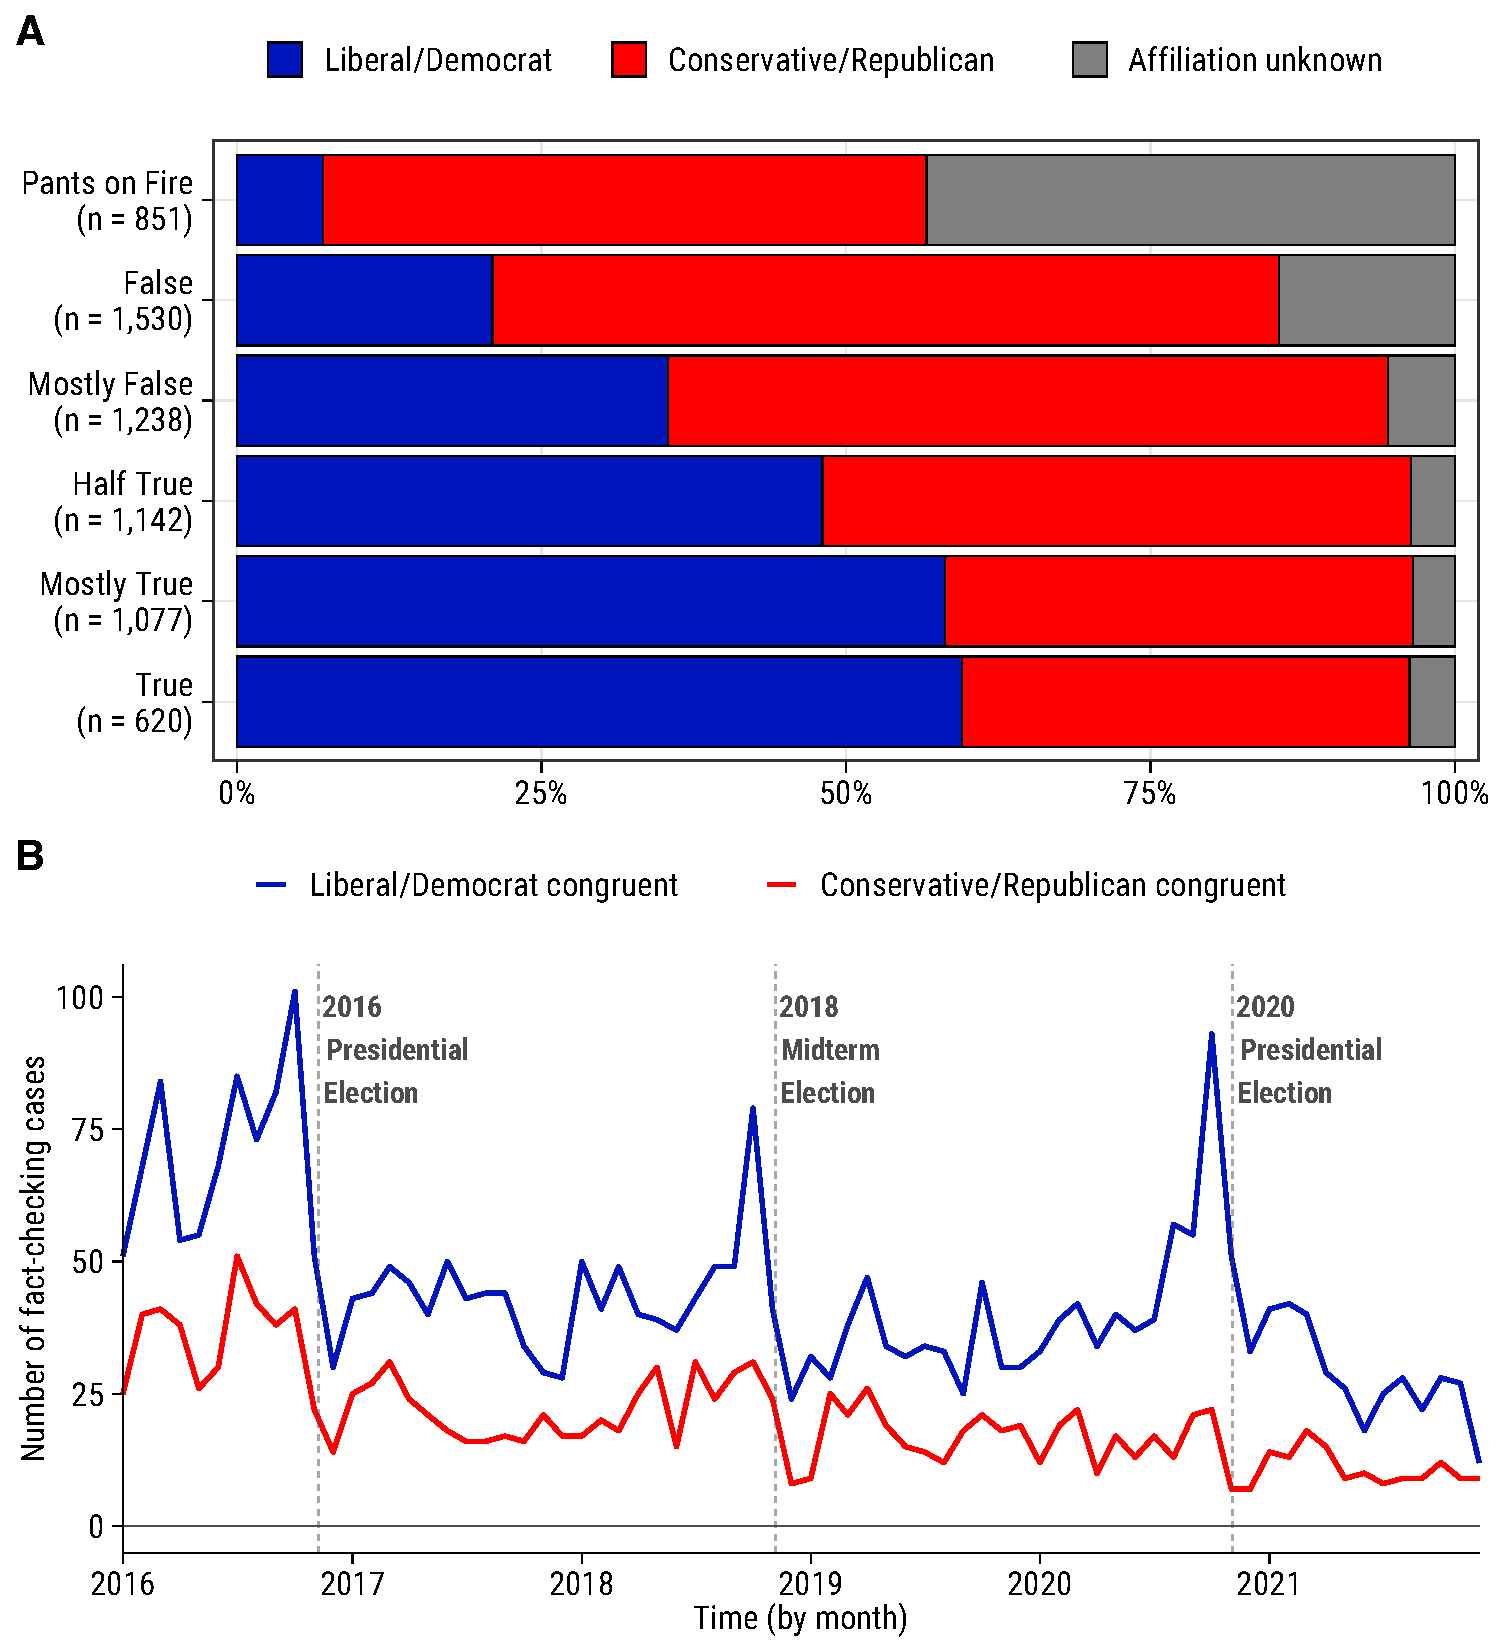
\includegraphics[width=1\textwidth]{../fig/merged_fig1.pdf}
\caption{Trends in political fact-checking by {\em PolitiFact}. (Panel A) Proportion of fact-checks sorted by the adjudication and party affiliation or political leaning of the target factual claim, conducted by {\em PolitiFact} from January 1, 2016, to December 31, 2021 ($N = 6,458$). (Panel B) Number of fact-checking articles that are congruent with Liberal/Democrats or Conservative/Republicans over time, presented on a monthly basis ($N = 4,598$).}
\label{fig:fig1}
\end{figure}

\newpage

\begin{figure}[!ht]
\centering
    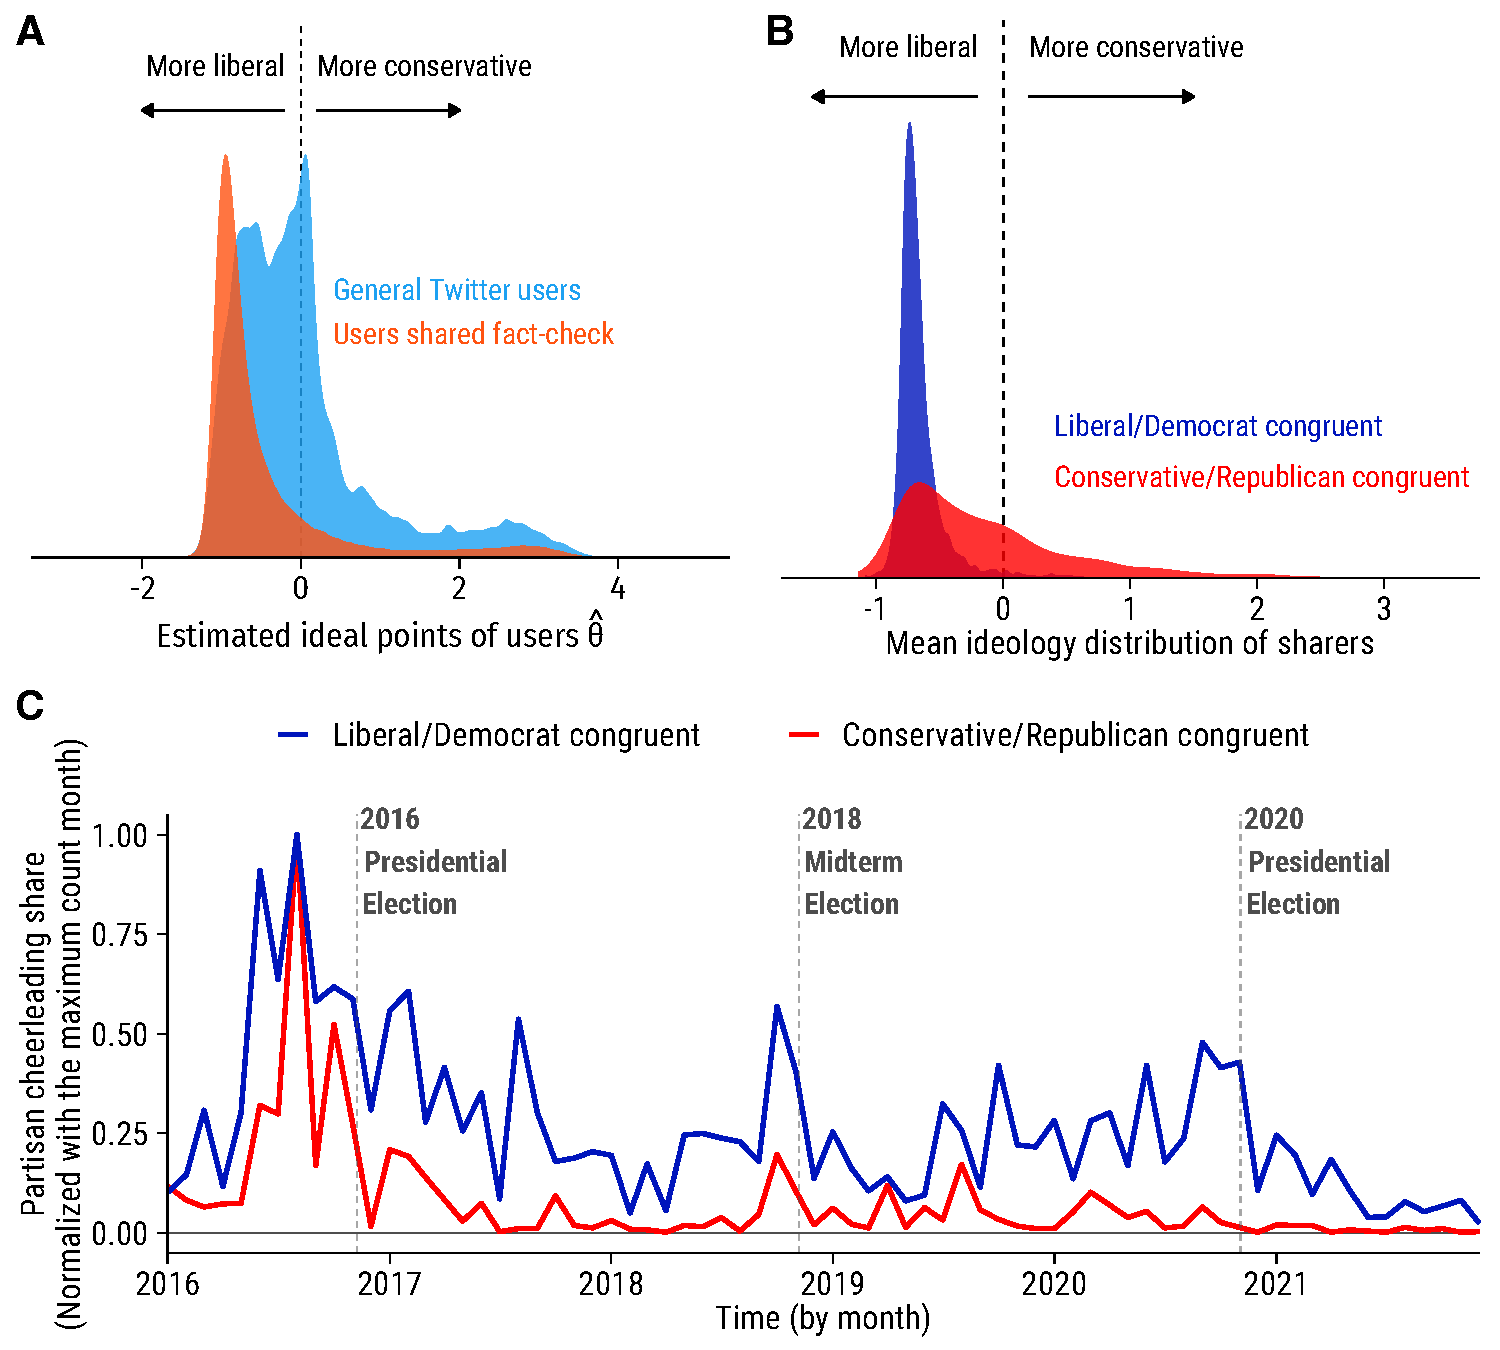
\includegraphics[width=\textwidth]{../fig/merged_fig2.pdf}
    \caption{Distribution of political fact-checking shares via social media. (Panel A) Comparative distribution of ideological scores for Twitter users ($N = 153,807$) who retweeted fact-checking posts and the overall Twitter user base ($N = 64,579,485$). (Panel B) Distribution of mean ideological scores of Twitter users who shared fact-checking posts, subdivided by each adjudication and the party affiliation/political leaning of the fact-check target. (Panel C) Timeline displaying the partisan selective sharing behavior of users from each political ideology (normalized by the maximum month's count in each ideology; $N_{\text{Max: Libs/Dem}} = 131,743; N_{\text{Max: Cons/Rep}} = 14,201$).}
    \label{fig:fig2}
\end{figure}

\newpage

\begin{figure}[!ht]
\centering
    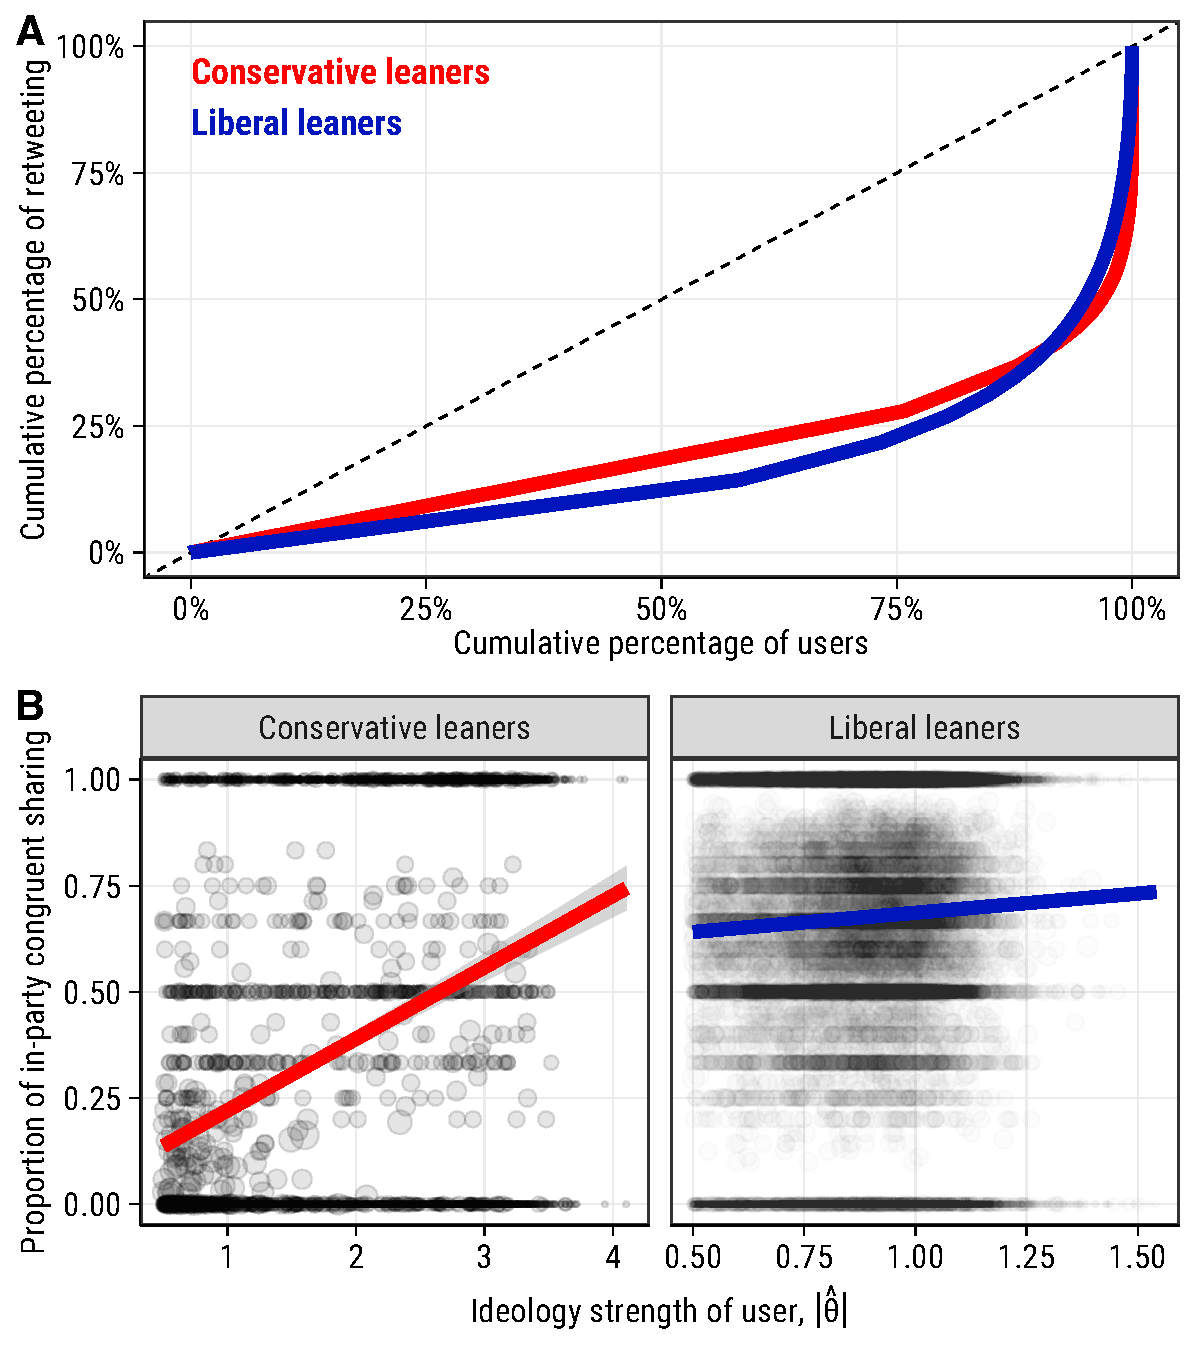
\includegraphics[width=\textwidth]{../fig/merged_fig3.pdf}
    \caption{Analysis of fact-check sharing behavior on Twitter based on user political ideology. (Panel A) A Lorenz curve illustrates the cumulative distribution of political fact-check shares across users, categorized by political ideology. (Panel B) Plot depicts the correlation between political ideology intensity and the proportion of selective fact-check sharing, with separate evaluations for Conservative-leaning and Liberal-leaning users. The fitted lines are estimated using the least squares method, where each unit is weighted according to its log-frequency of sharing.}
    \label{fig:fig3}
\end{figure}



\end{document}
